\documentclass[a4paper, 12pt]{book} % Classe do documento

% Pacotes básicos
\usepackage[utf8]{inputenc}   % Codificação de caracteres
\usepackage[T1]{fontenc}      % Codificação de fonte
\usepackage[portuguese]{babel} % Idioma do documento
\usepackage{amsthm, amsmath, amssymb} % Pacotes para matemática
\usepackage{graphicx}         % Inclusão de imagens
\usepackage{hyperref}         % Hiperlinks
\usepackage{tcolorbox}        % Caixas coloridas
\usepackage{lipsum}           % Gera texto de exemplo (remover após uso)
\usepackage{mdframed}
\usepackage{tabularx} % Adicione esta linha no preâmbulo
\usepackage{listings}
\usepackage{xcolor}
\usepackage{xurl}
\usepackage{booktabs}
\usepackage{tabularx}

\newtheorem{example}{Exemplo}[section]  % numera Exemplo dentro da seção

\newtheorem{exercicio}{Exercício}[chapter]

\usepackage{tikz}
\usetikzlibrary{shapes.geometric, arrows, fit}

\tikzstyle{block} = [rectangle, draw, fill=blue!20, text width=6em, text centered, rounded corners, minimum height=3em]
\tikzstyle{line} = [draw, -latex']
\tikzstyle{io} = [trapezium, trapezium left angle=70, trapezium right angle=110, draw, fill=green!20, minimum height=3em, text centered]

\setcounter{tocdepth}{1}

% Configurações de aparência
\hypersetup{
    colorlinks=true,
    linkcolor=black,
    urlcolor=black,
    pdftitle={Introdução à Programação},
    pdfauthor={Márcio Moretto Ribeiro},
}


% Título e autor
\title{Algoritmos e Estruturas de Dados 2\\ Tabelas de hash, árvores de busca e grafos}
\author{Márcio Moretto Ribeiro}
\date{\today} % Data automática

% Definir cores para o highlight
\definecolor{keywordcolor}{rgb}{0.5,0,0.5}  % Roxo para keywords
\definecolor{commentcolor}{rgb}{0,0.6,0}    % Verde para comentários
\definecolor{stringcolor}{rgb}{0.6,0,0}     % Vermelho para strings

\renewcommand{\lstlistingname}{Programa}

% Configuração do lstlisting para a linguagem C
\lstset{
    inputencoding=utf8,
    extendedchars=true,
    literate={á}{{\'a}}1 {é}{{\'e}}1 {í}{{\'i}}1 {ó}{{\'o}}1 {ú}{{\'u}}1
             {â}{{\^a}}1 {ê}{{\^e}}1 {î}{{\^i}}1 {ô}{{\^o}}1 {û}{{\^u}}1
             {ã}{{\~a}}1 {õ}{{\~o}}1 {ç}{{\c{c}}}1 {Á}{{\'A}}1 {É}{{\'E}}1
             {Í}{{\'I}}1 {Ó}{{\'O}}1 {Ú}{{\'U}}1 {Â}{{\^A}}1 {Ê}{{\^E}}1
             {Î}{{\^I}}1 {Ô}{{\^O}}1 {Û}{{\^U}}1 {Ã}{{\~A}}1 {Õ}{{\~O}}1
             {Ç}{{\c{C}}}1 {à}{{\`a}}1 {À}{{\`A}}1,
    language=C,                   % Linguagem C
    basicstyle=\ttfamily\small,   % Fonte monospace como verbatim
    keywordstyle=\color{keywordcolor}\bfseries, % Cor e negrito para keywords
    commentstyle=\color{commentcolor}\itshape,  % Cor e itálico para comentários
    stringstyle=\color{stringcolor},            % Cor para strings
    numbers=left,                 % Números de linha à esquerda
    numberstyle=\tiny\color{gray},% Estilo dos números de linha
    stepnumber=1,                 % Numeração de linha a cada linha
    tabsize=4,                    % Tamanho do tab
    showstringspaces=false,       % Não mostrar espaços em strings
    frame=single,                 % Coloca uma borda ao redor do código
    breaklines=true,              % Quebra linhas longas automaticamente
    captionpos=b,                 % Posição da legenda abaixo do código
}

\begin{document}

% Definindo o novo ambiente com título parametrizado
\newenvironment{extra}[1]
{
    \section{#1*}
     \begin{mdframed}[
        linewidth=0pt,
        backgroundcolor=blue!5,
    ]
}
{
    \end{mdframed}
}

% Capa
\maketitle
\tableofcontents

% Capítulo de introdução
\chapter{Introdução}

Estruturas de dados e algoritmos são os pilares fundamentais da ciência da computação. 
Enquanto algoritmos são sequências finitas de instruções bem definidas para resolver um problema ou realizar uma tarefa, estruturas de dados são formas de organizar, armazenar e acessar informações de maneira eficiente. 
Juntos, eles permitem que possamos resolver problemas complexos de forma sistemática, com clareza, precisão e eficiência. 
O mesmo problema pode ser abordado por diferentes algoritmos, e a escolha da estrutura de dados adequada muitas vezes determina o desempenho final da solução.

Compreender estruturas de dados e algoritmos é essencial para escrever programas corretos, legíveis e eficientes. 
Saber quando usar uma tabela de dispersão em vez de uma lista, ou uma árvore balanceada em vez de um vetor ordenado, é o que distingue uma solução ingênua de uma solução robusta e escalável. 
Além disso, a análise de algoritmos -- tanto no pior caso quanto em média -- fornece ferramentas para comparar alternativas e justificar decisões de projeto. 
Estudar esses temas é, portanto, um exercício de precisão lógica, mas também de criatividade na construção de soluções.

Estas notas foram elaboradas para acompanhar a disciplina e pressupõem que os alunos já tenham familiaridade com os fundamentos da análise de algoritmos -- como notação assintótica, complexidade de tempo e espaço, e noções básicas de recursão --, conteúdos geralmente abordados na disciplina {\em Introdução à Análise de Algoritmos}. 
Também se espera conhecimento prévio sobre estruturas de dados elementares, como vetores, listas ligadas, pilhas e filas, que são introduzidas em {\em Algoritmos e Estruturas de Dados 1}.

Nesta disciplina, o foco será o estudo de três classes centrais de estruturas de dados: tabelas de dispersão (hashes), árvores de busca e grafos. 
Esses temas serão tratados do ponto de vista conceitual e prático, com ênfase na análise de desempenho e nas aplicações típicas de cada estrutura. 
O objetivo é proporcionar uma base sólida que permita aos alunos projetar, implementar e analisar algoritmos eficientes para problemas que envolvem organização e busca de informação.

Nesta apostila, as estruturas de dados serão apresentadas inicialmente de forma abstrata, por meio de especificações em termos de Tipos Abstratos de Dados (TADs), seguidas por implementações em pseudocódigo e em linguagem C. 
A descrição abstrata permite compreender a funcionalidade esperada de cada estrutura sem se comprometer com detalhes de implementação, promovendo uma visão mais clara e geral. 
O pseudocódigo, por sua vez, serve como ponte entre a abstração conceitual e a codificação concreta, permitindo expressar os algoritmos de maneira legível e independente de linguagem. 
As implementações em C buscam fornecer uma visão prática e eficiente, permitindo ao aluno experimentar diretamente com os conceitos em exercícios e projetos.

Nesta apostila, os conteúdos são organizados em doze capítulos, acompanhando a sequência didática da disciplina. 
Iniciamos com uma introdução ao conceito de Tipos Abstratos de Dados (TADs), com ênfase no TAD dicionário e em suas duas variações principais: o dicionário simples e o dicionário ordenado. 
Em seguida, tratamos das tabelas de dispersão e funções de hash, abordando o conceito de função de dispersão, o fator de carga e aplicações como verificação de duplicatas e contagem de frequência.

Os capítulos seguintes se dedicam a técnicas de tratamento de colisões em tabelas de hash, incluindo encadeamento e sondagem linear, com menções a estratégias mais avançadas como sondagem quadrática e duplo hash. 
Também discutimos o desempenho dessas estruturas, analisando casos médios e piores, e revisitamos listas ligadas como suporte para algumas implementações.

Na segunda parte do curso, o foco se volta para árvores. 
Iniciamos pelas árvores binárias de busca, estudando sua implementação e uso como dicionários ordenados. 
Em seguida, apresentamos três variantes de árvores balanceadas: 
as árvores AVL, as árvores B (adequadas para acesso em disco) e as árvores vermelho-preto, que realizam balanceamento automático por meio de marcações nos nós.

A última parte da apostila é dedicada aos grafos. 
Apresentamos os conceitos fundamentais e representações possíveis, com exemplos de aplicações reais. 
Estudamos algoritmos de busca em grafos, como busca em largura (BFS) e busca em profundidade (DFS), e algoritmos para cálculo de caminhos mínimos, incluindo Dijkstra e Bellman-Ford. 
Encerramos com os algoritmos de Kruskal e Prim para obtenção de árvores geradoras mínimas, fundamentados no teorema do corte.

\section*{Objetivos}

O principal objetivo desta disciplina é aprofundar o conhecimento dos alunos sobre estruturas de dados e algoritmos, com foco na escolha e implementação de representações eficientes para problemas computacionais complexos. 
Pretende-se desenvolver a capacidade de raciocínio algorítmico, aliando clareza conceitual à análise crítica de desempenho.

Especificamente, ao final da disciplina, espera-se que o aluno seja capaz de:
\begin{itemize}
  \item Compreender e implementar estruturas de dados fundamentais como tabelas de dispersão, árvores de busca e grafos;
  \item Avaliar a eficiência de algoritmos em diferentes contextos, utilizando ferramentas de análise assintótica;
  \item Reconhecer padrões de problemas e selecionar estruturas e algoritmos adequados para resolvê-los;
  \item Aplicar os conceitos estudados em implementações práticas, com ênfase na correção, clareza e desempenho do código.
\end{itemize}

\section*{Bibliografia}

\begin{itemize}
  \item Goodrich \& Tamassia. {\em Estruturas de Dados e Algoritmos em Java} (Bookman, 2007).
  \item Sedgewick \& Wayne. {\em Algorithms, 4th Edition}.
\end{itemize}


\chapter{Tipos Abstratos de Dados (TADs)}

Quando programamos, é comum precisarmos agrupar dados e definir operações que possam ser realizadas sobre eles. 
Por exemplo, ao trabalhar com uma pilha de objetos, queremos adicionar ou remover um item do topo -- e, nesse contexto, o que nos interessa não é como os dados estão armazenados internamente, mas sim o comportamento da estrutura. 
Essa distinção entre o que uma estrutura faz e como ela faz é o ponto de partida para o conceito de Tipo Abstrato de Dado (TAD).

Um TAD é uma especificação formal de um conjunto de dados e das operações que podem ser realizadas sobre ele, independentemente da forma como essas operações são implementadas. 
Ao utilizar um TAD, o foco está no comportamento da estrutura -- nas operações disponíveis e em suas propriedades --, e não nos detalhes técnicos de código ou armazenamento. 
Isso permite que o programador raciocine de forma mais clara sobre o problema que está resolvendo, sem se distrair com questões de implementação.

Essa separação traz diversas vantagens. 
A principal delas é a modularidade: podemos dividir um programa em partes independentes, em que cada módulo (ou TAD) tem uma responsabilidade bem definida. Isso torna o código mais organizado, mais fácil de entender, de testar e de manter. 
Outra vantagem importante é a reutilização: um TAD bem projetado pode ser empregado em diferentes programas e contextos, sem a necessidade de reescrever sua lógica.

A essência de um TAD está na separação entre a definição lógica da estrutura e sua implementação concreta. 
Em vez de manipularmos diretamente a forma como os dados estão organizados na memória — como ocorre na programação estruturada tradicional —, interagimos apenas com um conjunto de funções que compõem a interface do TAD. 
Essas funções são as únicas autorizadas a acessar e modificar a estrutura interna dos dados. 
Essa restrição é fundamental: garante que todo acesso e modificação passem por um canal controlado, que pode impor regras e preservar invariantes. 
Essa abordagem lembra a forma como lidamos com funções em matemática: sabemos o que elas fazem, quais são suas entradas e saídas, mas não precisamos conhecer os detalhes internos de seu funcionamento para utilizá-las corretamente.

Ao longo desta apostila, utilizaremos TADs para representar estruturas como listas, dicionários, filas, árvores e grafos. 
Em cada caso, começaremos pela especificação abstrata -- ou seja, pela definição das operações disponíveis e de como elas devem se comportar -- e, em seguida, discutiremos possíveis implementações concretas. 
Essa metodologia permite entender a estrutura conceitualmente antes de mergulhar nos detalhes técnicos de sua construção.

\section{Dicionário Simples}

O TAD Dicionário representa uma coleção de pares chave--valor. Seu objetivo é permitir o armazenamento e a recuperação eficiente de informações associadas a uma chave. 
No caso do dicionário simples, as chaves são distintas -- ou seja, não há repetições --, e o conjunto de operações é focado na manipulação desse mapeamento básico.

Do ponto de vista abstrato, um dicionário simples oferece as seguintes operações fundamentais:

\begin{itemize}
  \item \texttt{criar()}: cria um dicionário vazio.
  
  \item \texttt{inserir(d, k, v)}: insere no dicionário \texttt{d} o par formado pela chave \texttt{k} e o valor \texttt{v}. Se a chave \texttt{k} já estiver presente, seu valor é substituído por \texttt{v}.
  
  \item \texttt{remover(d, k)}: remove do dicionário \texttt{d} o par associado à chave \texttt{k}. Se a chave não estiver presente, nenhuma alteração é feita.
  
  \item \texttt{buscar(d, k)}: retorna o valor associado à chave \texttt{k}, caso ela esteja presente no dicionário. Se a chave não existir, a operação indica ausência (por exemplo, retornando \texttt{null} ou um valor especial).
  
  \item \texttt{tamanho(d)}: retorna o número de pares armazenados no dicionário.
  
  \item \texttt{vazio(d)}: indica se o dicionário está vazio.
\end{itemize}

Essas operações definem o comportamento esperado da estrutura, sem especificar como os dados são armazenados internamente. 
A implementação pode variar -- por exemplo, pode-se usar listas, tabelas de dispersão (hash) ou árvores de busca --, mas o comportamento das funções deve seguir essa especificação. 
Essa separação permite ao programador utilizar o dicionário como uma ferramenta, sem precisar conhecer sua estrutura interna.

Nas próximas seções, estudaremos diferentes formas de implementar esse TAD, analisando os custos de cada operação e as vantagens de cada abordagem conforme o contexto de uso.


\subsection{Interface em C}

A seguir, apresentamos a interface do TAD Dicionário, definida em C como um arquivo de cabeçalho (dicionario.h). 
Essa interface descreve o conjunto de operações disponíveis para quem deseja utilizar um dicionário simples, sem revelar os detalhes da sua implementação. 
O uso de tipos opacos e ponteiros para funções permite que diferentes implementações (por exemplo, usando listas, tabelas de dispersão ou árvores) possam ser utilizadas de forma intercambiável, desde que respeitem o mesmo contrato.

\begin{lstlisting}[language=C, caption={Interface do TAD Dicionário}, label={lst:dicionario-h}]
#ifndef dic_H
#define dic_H

typedef const char* Chave;
typedef void* Valor;

// Tipo opaco para o dicionário
typedef struct Dicionario Dicionario;

// Interface do TAD
Dicionario* dic_criar();
void dic_inserir(Dicionario* d, Chave k, Valor v);
void dic_remover(Dicionario* d, Chave k);
Valor dic_buscar(Dicionario* d, Chave k);
int dic_tamanho(Dicionario* d);
int dic_vazio(Dicionario* d);
void dic_destruir(Dicionario* d);

#endif
\end{lstlisting}

Vamos analisar os principais elementos dessa interface:

\begin{itemize}
\item \verb|typedef const char* Chave;| define o tipo das chaves como cadeias de caracteres constantes. 
Em implementações reais, poderíamos generalizar esse tipo com ponteiros para funções de comparação ou usar um tipo genérico.

\item \verb|typedef void* Valor;| indica que os valores armazenados são genéricos, acessados como ponteiros opacos. 
Isso torna o dicionário flexível, podendo armazenar qualquer tipo de dado, desde que convertido para \texttt{void*}.

\item \verb|typedef struct Dicionario Dicionario;| declara um tipo opaco: o conteúdo interno da estrutura \texttt{Dicionario} não é revelado ao usuário do TAD. 
Isso reforça a ideia de encapsulamento -- o usuário interage com o dicionário apenas por meio das funções declaradas.

\item \verb|Dicionario* dic_criar();| aloca e retorna um novo dicionário vazio.

\item \verb|void dic_inserir(...);| insere um par chave–valor. Se a chave já existir, o valor anterior é substituído.

\item \verb|void dic_remover(...);| remove do dicionário o par associado à chave fornecida.

\item \verb|Valor dic_buscar(...);| retorna o valor associado a uma chave, ou \texttt{NULL} caso a chave não esteja presente.

\item \verb|int dic_tamanho(...);| retorna o número de elementos armazenados.

\item \verb|int dic_vazio(...);| retorna 1 se o dicionário estiver vazio, ou 0 caso contrário.

\item \verb|void dic_destruir(...);| libera toda a memória associada ao dicionário.
\end{itemize}

Essa interface oferece um conjunto consistente e mínimo de operações para manipular dicionários, mantendo a separação entre a especificação e a implementação. 
A estrutura interna pode ser alterada sem afetar o código dos usuários do TAD, desde que as funções mantenham o comportamento descrito.

\subsection{Exemplo de uso}

A seguir, mostramos um exemplo simples de como utilizar o TAD Dicionário. 
O programa cria um dicionário, insere dois pares chave–valor, busca um dos valores, remove uma das chaves e verifica se a remoção foi bem-sucedida. 
Ao final, a memória alocada é liberada com a operação de destruição.

\begin{lstlisting}[language=C, caption={Exemplo de uso do TAD Dicionário}, label={lst:exemplo-uso}]
#include <stdio.h>
#include <stdlib.h>
#include "dicionario.h"

int main() {
	Dicionario* d = dic_criar();

	dic_inserir(d, "chave1", "valor1");
	dic_inserir(d, "chave2", "valor2");

	printf("%s\n", (char*) dic_buscar(d, "chave1")); // imprime valor1

	dic_remover(d, "chave1");

	if (dic_buscar(d, "chave1") == NULL)
    	printf("chave1 removida\n");

	dic_destruir(d);
	return 0;
}
\end{lstlisting}

Vamos destacar alguns pontos importantes sobre esse código:

\begin{itemize}
\item A função \verb|dic_criar()| aloca dinamicamente um novo dicionário e retorna um ponteiro para ele.
\item As strings passadas como chave e valor neste exemplo são literais de string (constantes). 
Como o tipo \verb|Valor| é genérico (\verb|void*|), precisamos fazer \verb|cast| para \verb|char*| ao imprimir.
\item A função \verb|dic_buscar()| retorna o valor associado à chave ou \verb|NULL| se a chave não estiver presente. Isso é usado para verificar se a remoção foi bem-sucedida.
\item Por fim, \verb|dic_destruir()| libera toda a memória alocada pelo dicionário.
\end{itemize}

Esse exemplo mostra como a interface permite manipular o dicionário de forma intuitiva, sem que o usuário precise conhecer a estrutura interna usada para armazenar os dados. 
A mesma interface pode ser usada com diferentes implementações, o que demonstra na prática a vantagem da abstração promovida pelo TAD.

\subsection{Implementação com Lista Ligada}

Como primeira forma concreta de implementar o TAD Dicionário, utilizamos uma lista ligada simples. 
Cada elemento da lista armazena um par chave–valor, bem como um ponteiro para o próximo elemento. Essa é uma estratégia simples e direta, adequada para conjuntos pequenos de dados ou para fins didáticos.

Nesta implementação com lista ligada, cada operação é realizada da seguinte forma:

\begin{itemize}
\item A inserção de um novo par chave–valor é feita sempre no início da lista.
\item Se a chave já existir, o valor correspondente é atualizado e a lista permanece inalterada em estrutura.
\item A busca percorre os nós da lista, do primeiro até encontrar a chave desejada ou chegar ao final.
\item A remoção também percorre a lista até localizar o nó com a chave desejada, ajustando os ponteiros para removê-lo.
\item A estrutura mantém um contador de elementos, permitindo obter o tamanho atual do dicionário de forma direta.
\item A verificação de dicionário vazio é feita consultando esse contador.
\end{itemize}

Essa organização permite uma implementação simples e clara, ideal como primeira aproximação do TAD Dicionário. 
A estrutura interna permanece escondida do usuário, que interage apenas por meio das funções da interface.

\begin{lstlisting}[language=C, caption={Implementação do TAD Dicionário com lista ligada}, label={lst:dicionario-lista}]
#include <stdio.h>
#include <stdlib.h>
#include <string.h>
#include "dicionario.h"

typedef struct No {
	Chave chave;
	Valor valor;
	struct No* prox;
} No;

struct Dicionario {
	No* primeiro;
	int tamanho;
};

Dicionario* dic_criar() {
	Dicionario* d = malloc(sizeof(Dicionario));
	d->primeiro = NULL;
	d->tamanho = 0;
	return d;
}

void dic_inserir(Dicionario* d, Chave k, Valor v) {
	No* atual = d->primeiro;
	while (atual != NULL) {
		if (strcmp(atual->chave, k) == 0) {
			atual->valor = v;
			return;
		}
		atual = atual->prox;
	}
	No* novo = malloc(sizeof(No));
	novo->chave = k;
	novo->valor = v;
	novo->prox = d->primeiro;
	d->primeiro = novo;
	d->tamanho++;
}

void dic_remover(Dicionario* d, Chave k) {
	No** pp = &d->primeiro;
	while (*pp != NULL) {
		if (strcmp((pp)->chave, k) == 0) {
			No temp = *pp;
			*pp = temp->prox;
			free(temp);
			d->tamanho--;
			return;
		}
		pp = &(*pp)->prox;
	}
}

Valor dic_buscar(Dicionario* d, Chave k) {
	No* atual = d->primeiro;
	while (atual != NULL) {
		if (strcmp(atual->chave, k) == 0) {
			return atual->valor;
		}
		atual = atual->prox;
	}
	return NULL;
}

int dic_tamanho(Dicionario* d) {
	return d->tamanho;
}

int dic_vazio(Dicionario* d) {
	return d->tamanho == 0;
}

void dic_destruir(Dicionario* d) {
	No* atual = d->primeiro;
	while (atual != NULL) {
		No* temp = atual;
		atual = atual->prox;
		free(temp);
	}
	free(d);
}
\end{lstlisting}

Essa implementação satisfaz todos os requisitos do TAD Dicionário: encapsula os dados, respeita a interface pública definida no arquivo \texttt{dicionario.h}, e pode ser substituída por outra (como uma baseada em tabela de dispersão ou árvore) sem alterar o código dos programas que usam o TAD.
Essa separação entre interface e implementação é o que torna os TADs uma ferramenta poderosa na construção de software modular e reutilizável.

\subsection{Análise de Eficiência da Implementação com Lista Ligada}

A implementação do TAD Dicionário com lista ligada é funcional e simples, mas sua eficiência depende diretamente do número de elementos armazenados. A seguir, avaliamos cada operação em termos do custo computacional no pior caso, considerando $n$ como o número de pares armazenados no dicionário.

\begin{itemize}
\item \textbf{\texttt{criar()}}
A criação do dicionário consiste na alocação de uma estrutura inicial com ponteiro nulo e contador zero.
\textbf{Custo:} $O(1)$

\item \textbf{\texttt{inserir(d, k, v)}}
Para inserir, é necessário primeiro percorrer a lista para verificar se a chave já existe. Se encontrar, o valor é atualizado. Caso contrário, um novo nó é inserido no início.
\textbf{Custo:} $O(n)$ no pior caso (quando a chave não está presente)

\item \textbf{\texttt{remover(d, k)}}
A remoção percorre a lista até encontrar a chave. Ao localizar o nó, ajusta os ponteiros e libera a memória.
\textbf{Custo:} $O(n)$ no pior caso

\item \textbf{\texttt{buscar(d, k)}}
A busca percorre os nós da lista, comparando cada chave até encontrar a desejada ou atingir o final.
\textbf{Custo:} $O(n)$ no pior caso

\item \textbf{\texttt{tamanho(d)}}
O tamanho é mantido por um contador atualizado a cada inserção ou remoção, portanto não exige varredura da lista.
\textbf{Custo:} $O(1)$

\item \textbf{\texttt{vazio(d)}}
A verificação se o dicionário está vazio consulta apenas o valor do contador.
\textbf{Custo:} $O(1)$

\item \textbf{\texttt{destruir(d)}}
A destruição percorre toda a lista e libera a memória de cada nó.
\textbf{Custo:} $O(n)$
\end{itemize}

A principal limitação dessa abordagem está nas operações que dependem da busca por uma chave (inserção, remoção e busca propriamente dita), que exigem varredura linear da lista. 
Mais adiante, exploraremos implementações que oferecem desempenho mais eficiente para essas operações, como tabelas de dispersão e árvores de busca.

\section{Dicionário Ordenado}

O TAD Dicionário Ordenado estende o TAD Dicionário Simples com operações que exploram a ordenação das chaves. 
Assume-se que as chaves pertencem a um conjunto em que existe uma relação de ordem total -- isto é, qualquer par de chaves pode ser comparado usando operadores como ``menor que'', ``maior que'', ou ``igual''.

O comportamento esperado das operações é o seguinte:

\begin{itemize}
\item \verb|menor(d)|: retorna a menor chave armazenada no dicionário \texttt{d}, ou indica ausência se o dicionário estiver vazio.

\item \verb|maior(d)|: retorna a maior chave armazenada no dicionário \texttt{d}, ou indica ausência se o dicionário estiver vazio.

\item \verb|anterior(d, k)|: retorna a maior chave armazenada que seja estritamente menor que \texttt{k}, ou indica ausência caso tal chave não exista.

\item \verb|posterior(d, k)|: retorna a menor chave armazenada que seja estritamente maior que \texttt{k}, ou indica ausência caso tal chave não exista.

\item \verb|visitar_em_ordem(d, f)|: percorre o dicionário \texttt{d} em ordem crescente de chave e aplica a função \texttt{f(k, v)} para cada par chave–valor armazenado.
\end{itemize}

Essas operações permitem, por exemplo, percorrer os dados em ordem crescente, implementar buscas intervalares (como ``todas as chaves entre a e b'') e construir algoritmos que dependem de vizinhanças ordenadas. 
A implementação dessas operações exige estruturas de dados que mantenham a ordem, como árvores binárias de busca.

\subsection*{Interface em C}

A interface do TAD Dicionário Ordenado é uma extensão da interface do dicionário simples. Se estivéssemos utilizando uma linguagem orientada a objetos, como Java ou C++, poderíamos definir o dicionário ordenado como uma subclasse do dicionário simples, herdando todas as operações básicas e adicionando apenas as operações específicas de ordenação.

Entretanto, como estamos implementando o TAD em C -- uma linguagem que não possui herança nem mecanismos nativos de orientação a objetos -- optamos por declarar explicitamente todas as operações, mesmo que algumas já existam na interface do dicionário simples. 
Essa repetição facilita a organização e deixa clara a assinatura completa da interface para quem vai utilizá-la.

Abaixo está uma possível definição da interface para o TAD Dicionário Ordenado:

\begin{lstlisting}[language=C, caption={Interface do TAD Dicionário Ordenado}, label={lst:dicionario-ordenado-h}]
#ifndef dic_ord_H
#define dic_ord_H

typedef const char* Chave;
typedef void* Valor;

typedef struct DicionarioOrdenado DicionarioOrdenado;

// Interface herdada do dicionário simples
DicionarioOrdenado* dic_ord_criar();
void dic_ord_inserir(DicionarioOrdenado* d, Chave k, Valor v);
void dic_ord_remover(DicionarioOrdenado* d, Chave k);
Valor dic_ord_buscar(DicionarioOrdenado* d, Chave k);
int dic_ord_tamanho(DicionarioOrdenado* d);
int dic_ord_vazio(DicionarioOrdenado* d);
void dic_ord_destruir(DicionarioOrdenado* d);

// Novas operações específicas da ordenação
Chave dic_ord_menor(DicionarioOrdenado* d);
Chave dic_ord_maior(DicionarioOrdenado* d);
Chave dic_ord_anterior(DicionarioOrdenado* d, Chave k);
Chave dic_ord_posterior(DicionarioOrdenado* d, Chave k);
void dic_ord_visitar_em_ordem(DicionarioOrdenado* d, void (*visita)(Chave, Valor));

#endif
\end{lstlisting}

Com essa interface, podemos implementar as funções do TAD Dicionário Ordenado usando diferentes estruturas de dados que mantêm os elementos ordenados — como árvores binárias de busca (que veremos a seguir). 
O usuário do TAD continua protegido da implementação interna, utilizando apenas os nomes das funções definidas na interface.

\subsection{Exemplo de uso}

A seguir, mostramos um exemplo básico de uso do TAD Dicionário Ordenado. 
O programa insere alguns pares chave–valor, exibe o menor e o maior elemento, e percorre o dicionário em ordem crescente.

\begin{lstlisting}[language=C, caption={Exemplo de uso do Dicionário Ordenado}, label={lst:uso-dicionario-ordenado}]
#include <stdio.h>
#include "dic_ord.h"

void imprimir(Chave k, Valor v) {
	printf("%s -> %s\n", k, (char*) v);
}

int main() {
	DicionarioOrdenado* d = dic_ord_criar();

	dic_ord_inserir(d, "joao", "Aluno");
	dic_ord_inserir(d, "ana", "Professora");
	dic_ord_inserir(d, "maria", "Coordenadora");

	printf("Menor chave: %s\n", dic_ord_menor(d));
	printf("Maior chave: %s\n", dic_ord_maior(d));

	Chave a = "maria";
	Chave ant = dic_ord_anterior(d, a);
	Chave pos = dic_ord_posterior(d, a);
	if (ant) printf("Anterior a %s: %s\n", a, ant);
	if (pos) printf("Posterior a %s: %s\n", a, pos);

	printf("\nElementos em ordem:\n");
	dic_ord_visitar_em_ordem(d, imprimir);

	dic_ord_destruir(d);
	return 0;
}
\end{lstlisting}

\textbf{Saída esperada:}
\begin{verbatim}
Menor chave: ana
Maior chave: maria
Anterior a maria: joao
Posterior a maria: (nada)

Elementos em ordem:
ana -> Professora
joao -> Aluno
maria -> Coordenadora
\end{verbatim}

Esse exemplo mostra como o TAD Dicionário Ordenado permite não apenas armazenar e recuperar valores por chave, mas também explorar relações de ordem entre as chaves, algo que não seria possível com a versão simples do TAD.

\part{Hash}
\chapter{Tabela de Dispersão}

No capítulo anterior, apresentamos o TAD dicionário, uma estrutura abstrata que associa chaves a valores por meio de operações como inserção, busca e remoção. 
Implementações simples usando listas ou vetores são funcionais, mas pouco eficientes: no pior caso, é necessário percorrer toda a estrutura para localizar uma chave, resultando em tempo linear por operação.

Tabelas de dispersão -- ou tabelas hash -- oferecem uma alternativa muito mais eficiente. 
Utilizando uma função de hash para mapear chaves diretamente a posições de uma tabela, é possível realizar essas operações em tempo constante no caso médio, desde que a função seja bem projetada e o fator de carga esteja controlado.

Essa eficiência torna as tabelas hash ideais para aplicações como:
\begin{itemize}
  \item verificação de duplicatas (por exemplo, ao filtrar elementos repetidos);
  \item contagem de frequência (como contar palavras em um texto);
  \item acesso rápido a dados indexados por identificadores (como nomes de usuário ou códigos de produto).
\end{itemize}

Tabelas hash estão presentes em praticamente todas as linguagens de programação modernas e são fundamentais para o desenvolvimento de sistemas rápidos e escaláveis. 
Nesta aula, daremos os primeiros passos para entendê-las.

Uma tabela de dispersão, ou \emph{hash table}, é uma estrutura de dados usada para associar chaves a valores. 
A ideia central é utilizar uma função de hash para transformar a chave (por exemplo, uma palavra, um número ou um identificador) em um índice de um vetor.
Esse índice indica a posição onde o valor correspondente deve ser armazenado ou recuperado.

A estrutura básica consiste em:
\begin{itemize}
  \item uma \emph{função de hash}, que transforma uma chave em um número inteiro;
  \item um \emph{vetor} (ou tabela) onde os valores são armazenados em posições indicadas pela função de hash.
\end{itemize}

Por exemplo, ao registrar a frequência de palavras em um texto, podemos usar a palavra como chave e sua contagem como valor. 
A função de hash transforma a palavra em um número que indica uma posição na tabela, onde a contagem será atualizada.

Esse mecanismo permite acessar os dados diretamente a partir da chave, sem a necessidade de percorrer toda a estrutura. 
A ideia é que chaves diferentes sejam distribuídas (ou ``dispersadas'') ao longo da tabela, ocupando posições distintas.

No entanto, pode acontecer de duas chaves diferentes serem transformadas pela função de hash no mesmo índice. 
Isso é chamado de \textbf{colisão}. 
Por exemplo, as palavras \texttt{``casa''} e \texttt{``amor''} podem acabar sendo associadas à mesma posição da tabela. 
A forma como lidar com colisões será discutida mais para frente no capítulo.

\section{Dicionário e Tabelas de Hash}

Como vimos no capítulo anterior, o ponto de vista abstrato de um dicionário simples envolve operações como \texttt{criar()}, \texttt{inserir()}, \texttt{remover()}, \texttt{buscar()}, \texttt{tamanho()} e \texttt{vazio()}. 
A ideia é manipular pares \texttt{(chave, valor)} de maneira eficiente, sem nos preocupar com os detalhes da implementação.

As tabelas de dispersão oferecem uma maneira concreta e eficiente de implementar esse TAD. 
A função de hash permite transformar uma chave \texttt{k} em um índice de um vetor, e esse índice determina a posição onde o par \texttt{(k, v)} será armazenado. 
Com isso, as operações fundamentais do dicionário podem ser implementadas da seguinte forma:

\begin{itemize}
  \item \texttt{criar()}: aloca um vetor (tabela) inicialmente vazio.
  
  \item \texttt{inserir(d, k, v)}: aplica a função de hash à chave \texttt{k} para determinar a posição na tabela, e insere o par \texttt{(k, v)} nessa posição.
  
  \item \texttt{remover(d, k)}: aplica a função de hash à chave \texttt{k} para localizar sua posição na tabela, e remove o par armazenado ali (caso exista).
  
  \item \texttt{buscar(d, k)}: aplica a função de hash à chave \texttt{k} e retorna o valor armazenado na posição correspondente.
\end{itemize}

As demais operações, como \texttt{tamanho()} e \texttt{vazio()}, podem ser implementadas com contadores auxiliares mantidos junto à estrutura.

Assim, uma tabela de hash concretiza o TAD dicionário a partir da ideia de associar chaves a posições calculadas por uma função de hash. 
Essa associação direta evita buscas lineares, tornando as operações mais ágeis, como veremos em detalhes nas próximas seções.

\section{Funções de Hash}

O elemento central de uma tabela de dispersão é a \emph{função de hash}. 
Ela é responsável por transformar uma chave arbitrária (como um número, uma palavra ou uma estrutura mais complexa) em um número inteiro que servirá como índice da tabela.

Formalmente, uma função de hash é uma função \texttt{h(k)} que recebe uma chave \texttt{k} e retorna um número inteiro entre \texttt{0} e \texttt{N -- 1}, onde \texttt{N} é o tamanho da tabela.

Para que a tabela funcione bem, é importante que a função de hash atenda a alguns requisitos:

\begin{itemize}
  \item \textbf{Determinismo:} a mesma chave deve sempre produzir o mesmo índice. 
  Isso é essencial para que seja possível recuperar os dados corretamente.
  
  \item \textbf{Distribuição uniforme:} as chaves devem ser espalhadas de forma razoavelmente uniforme pelos índices da tabela, evitando que muitas chaves sejam mapeadas para a mesma posição.
  
  \item \textbf{Simplicidade computacional:} a função deve ser fácil de calcular, já que será chamada com frequência nas operações de inserção, busca e remoção.
\end{itemize}

\subsection*{Exemplos simples}

\begin{itemize}
  \item \textbf{Hash para inteiros:} uma função simples e comum é usar o operador módulo:
  \[
  h(x) = x \bmod N
  \]
  onde \texttt{N} é o tamanho da tabela. Por exemplo, se \texttt{N = 10} e \texttt{x = 37}, temos \texttt{h(37) = 7}.
  
  \item \textbf{Hash para strings:} uma estratégia básica é usar o valor numérico dos caracteres da string (por exemplo, o código ASCII) com pesos:
  \[
  h(s) = (c_0 + 31 \cdot c_1 + 31^2 \cdot c_2 + \dots + 31^{n-1} \cdot c_{n-1}) \bmod N
  \]
  onde \texttt{c\_i} é o código do $i$-ésimo caractere da string. O número 31 é uma base comumente usada por ser um número primo pequeno.
\end{itemize}

Esses exemplos ilustram a ideia geral de funções de hash. 
O tratamento de colisões -- quando duas chaves diferentes resultam no mesmo índice -- será discutido nas próximas seções.

\section{Fator de Carga}

Ao construir uma tabela de dispersão, é importante controlar a quantidade de elementos que estamos armazenando em relação ao tamanho da tabela. 
Esse controle é feito por meio de um valor chamado \emph{fator de carga}.

\subsection*{Definição}

O fator de carga de uma tabela de hash é definido pela razão:
\[
\alpha = \frac{n}{m}
\]
onde:
\begin{itemize}
  \item \texttt{n} é o número de elementos armazenados na tabela;
  \item \texttt{m} é o número total de posições disponíveis (ou seja, o tamanho do vetor).
\end{itemize}

Esse valor nos dá uma ideia de quão ``cheia'' está a tabela.

\subsection*{Impacto sobre o desempenho}

Quanto maior o fator de carga, maior a chance de ocorrerem colisões -- ou seja, de duas ou mais chaves serem mapeadas para a mesma posição da tabela. 
Quando muitas colisões ocorrem, as operações de busca, inserção e remoção tendem a ficar mais lentas, pois passam a depender de mecanismos extras para resolver conflitos.

Por outro lado, manter a tabela com muitas posições vazias (isto é, um fator de carga muito pequeno) pode desperdiçar memória.

\subsection*{Estratégias para manter um bom fator de carga}

Para manter o desempenho da tabela em níveis aceitáveis, costuma-se adotar estratégias como:

\begin{itemize}
  \item \textbf{Escolher um tamanho inicial adequado} para a tabela, levando em conta a estimativa de número de elementos.
  
  \item \textbf{Monitorar o fator de carga} durante as operações, e realizar um \emph{redimensionamento} (ou \emph{rehashing}) quando ele ultrapassa um certo limite.
  
  \item \textbf{Utilizar tamanhos de tabela primos} pode ajudar a reduzir padrões indesejados na distribuição das chaves.
\end{itemize}

Nos próximos capítulos, veremos como essas estratégias se aplicam na prática e como diferentes métodos de resolução de colisão se comportam com diferentes fatores de carga.

\section{Exemplos de Funções de Hash}

Para entender na prática como diferentes funções de hash se comportam, realizamos um experimento simples: escolhemos um conjunto realista de chaves e aplicamos diversas funções sobre ele, observando a distribuição resultante em uma tabela de dispersão com tamanho fixo.

\subsection*{O conjunto de chaves: palavras de \emph{O Arquipélago Gulag}}

Utilizamos como base o livro \emph{O Arquipélago Gulag}, de Aleksandr Soljenítsin, uma das principais obras do século XX sobre o sistema de campos de trabalho forçado da União Soviética. 
O livro combina testemunhos pessoais, documentos históricos e análise política, e se tornou um símbolo da denúncia dos regimes totalitários.

A partir do texto completo, extraímos todas as palavras distintas -- ao todo, \textbf{22.077 palavras únicas}. 
Esse conjunto é representativo por conter vocabulário natural, com repetições, prefixos, sufixos e estruturas linguísticas recorrentes.

\subsection*{O experimento}

Para cada função de hash analisada, aplicamos a seguinte metodologia:

\begin{enumerate}
  \item Cada palavra foi convertida em um número inteiro usando a função de hash em questão.
  \item Esse número foi reduzido ao intervalo $[0, N - 1]$ com uma operação de módulo, usando $N = 1000$ (tabela pequena) e $N = 50000$ (tabela grande).
  \item Contamos quantas palavras foram mapeadas para cada índice da tabela.
  \item Analisamos a distribuição: número de colisões, posições vazias, e o maior acúmulo de palavras em um único índice.
\end{enumerate}

\subsection*{Objetivo}

O objetivo do experimento é ilustrar de forma empírica como diferentes funções de hash afetam a distribuição das chaves na tabela. 
Algumas funções aparentemente simples podem gerar distribuições desbalanceadas, com muitas colisões e uso desigual das posições. Outras, mesmo com implementações simples, apresentam desempenho muito melhor.

Nos exemplos seguintes, comparamos duas funções:

\begin{itemize}
  \item uma função baseada na \textbf{soma dos caracteres} (muito simples, e com desempenho ruim);
  \item a função \textbf{polinomial com base 31}, usada em muitas bibliotecas padrão;
\end{itemize}

Essa comparação ajudará a visualizar, com dados reais, os impactos concretos de uma boa ou má escolha de função de hash.

\subsection*{Função baseada na soma dos caracteres}

A primeira função que analisamos é extremamente simples: ela calcula a soma dos valores numéricos dos caracteres da string, e então aplica o operador módulo com o tamanho da tabela:
\[
h(s) = \left( \sum_{i=0}^{n-1} \texttt{ord}(s_i) \right) \bmod N
\]
Essa função é fácil de implementar e computacionalmente barata. No entanto, ela apresenta sérios problemas quando aplicada a dados reais como palavras de um texto.

\begin{example}
Considere a palavra \texttt{programador}. 
Vamos calcular o valor de hash utilizando a função baseada na soma dos códigos dos caracteres.

Os valores ASCII dos caracteres são:

\begin{center}
\begin{tabular}{c|c}
Letra & Código \\
\hline
p & 112 \\
r & 114 \\
o & 111 \\
g & 103 \\
r & 114 \\
a & 97 \\
m & 109 \\
a & 97 \\
d & 100 \\
o & 111 \\
r & 114 \\
\end{tabular}
\end{center}


Somando os valores:
\[
112 + 114 + 111 + 103 + 114 + 97 + 109 + 97 + 100 + 111 + 114 = 1.182
\]

Se estivermos usando uma tabela com $N = 1000$ posições, o valor da função será:
\[
h(\texttt{programador}) = 1182\ \bmod\ 1000 = 182
\]

Assim, a palavra \texttt{programador} seria armazenada na posição 182 da tabela.

Esse exemplo mostra que, mesmo com palavras um pouco maiores, a soma raramente ultrapassa 1500 — o que explica por que funções baseadas apenas na soma tendem a ocupar uma faixa muito estreita da tabela.

\end{example}

\subsubsection*{Resultados com $N = 1000$}

Aplicamos essa função às 22.077 palavras distintas de \emph{O Arquipélago Gulag}, usando uma tabela de tamanho $N = 1000$. 
Os resultados mostraram uma distribuição bastante desigual:

\begin{itemize}
  \item \textbf{17 posições} da tabela ficaram completamente vazias;
  \item Algumas posições armazenaram mais de \textbf{60 palavras diferentes};
  \item O número total de colisões foi elevado em comparação com outras funções;
  \item Muitas palavras distintas foram mapeadas para o mesmo índice.
\end{itemize}

\begin{figure}[h]
\centering
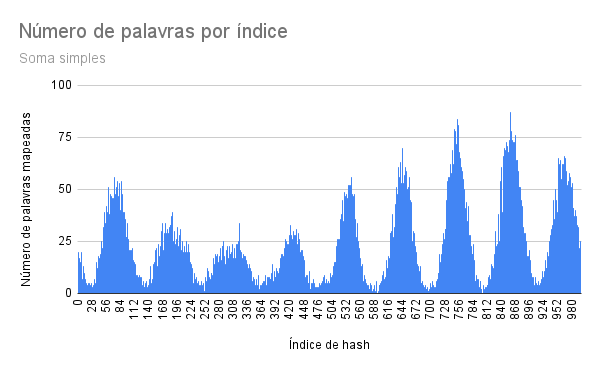
\includegraphics[width=0.9\textwidth]{soma_simples.png}
\caption{Distribuição de palavras distintas por índice da tabela usando a função de hash baseada na soma dos caracteres.}
\end{figure}

\subsubsection*{Resultados com $N = 50000$}

Repetimos o experimento com a função baseada na soma dos caracteres, agora utilizando uma tabela com $N = 50000$ posições. 
Apesar do aumento expressivo no tamanho da tabela, os resultados permaneceram insatisfatórios:

\begin{itemize}
  \item \textbf{48.600 posições} da tabela ficaram completamente vazias;
  \item A maior carga observada em um único índice foi novamente de \textbf{87 palavras distintas};
  \item O número total de colisões foi de \textbf{20.677}, praticamente igual ao observado com $N = 1000$;
  \item Apenas uma pequena faixa inicial da tabela foi efetivamente utilizada -- a maioria dos índices jamais recebeu qualquer palavra.
\end{itemize}

Esse comportamento ocorre porque a função de hash baseada na soma dos caracteres gera valores relativamente baixos: como a maioria das palavras tem entre 4 e 15 letras e utiliza caracteres com códigos entre 97 e 122 (no caso de letras minúsculas), a soma total raramente ultrapassa 1500. 
Com isso, todos os valores de hash produzidos se concentram nos primeiros mil ou dois mil índices da tabela. 
Os demais índices -- mais de 90\% da tabela -- simplesmente não são utilizados. 
Isso evidencia uma das principais falhas dessa função: sua incapacidade de aproveitar o espaço disponível, mesmo quando a tabela é grande.


\subsubsection*{Por que essa função falha?}

Apesar de ser válida como função no sentido técnico (é determinística e retorna um valor inteiro), essa função é inadequada para uso prático em tabelas de dispersão. 
Os principais problemas são:

\begin{itemize}
  \item \textbf{Ignora a ordem dos caracteres:} palavras como \texttt{amor} e \texttt{roma} têm o mesmo valor de hash.
  \item \textbf{Alta redundância linguística:} palavras com estruturas semelhantes (prefixos, sufixos, letras de mesmo valor) tendem a cair nas mesmas posições.
  \item \textbf{Pouca difusão:} pequenas mudanças na entrada resultam em mudanças pequenas no hash.
\end{itemize}

Esse exemplo mostra que a escolha da função de hash tem impacto direto sobre a eficiência da tabela: funções simples demais podem gerar um número elevado de colisões, comprometendo o desempenho das operações básicas.

\subsection*{Função polinomial com base 31}

A segunda função que analisamos é baseada em um cálculo polinomial clássico, que atribui pesos crescentes aos caracteres da string conforme sua posição:
\[
h(s) = (c_0 + 31 \cdot c_1 + 31^2 \cdot c_2 + \dots + 31^{n-1} \cdot c_{n-1}) \bmod N
\]
onde $c_i$ representa o valor numérico do $i$-ésimo caractere. Essa função leva em conta a ordem dos caracteres, o que a torna mais sensível a variações entre palavras diferentes.

\begin{example}
\subsubsection*{Exemplo ilustrativo}

Vamos agora calcular o valor da função de hash polinomial com base 31 para a palavra \texttt{programador}. Essa função considera a ordem dos caracteres e aplica pesos exponenciais:

\[
h(s) = (c_0 + 31 \cdot c_1 + 31^2 \cdot c_2 + \dots + 31^{n-1} \cdot c_{n-1}) \bmod N
\]

Para \texttt{programador}, com $N = 1000$, temos os seguintes valores ASCII:

\begin{center}
\begin{tabular}{c|c|l}
Letra & Código & Peso \\
\hline
p & 112 & $31^0$ = 1 \\
r & 114 & $31^1$ = 31 \\
o & 111 & $31^2$ = 961 \\
g & 103 & $31^3$ = 29.791 \\
r & 114 & $31^4$ = 923.521 \\
a & 97 & $31^5$ = 28.628.151 \\
m & 109 & $31^6$ = 887.472.681 \\
a & 97 & $31^7$ = 27.511.653.111 \\
d & 100 & $31^8$ = 852.861.246.441 \\
o & 111 & $31^9$ = 26.438.698.639.671 \\
r & 114 & $31^{10}$ = 820.599.658.829.801 \\
\end{tabular}
\end{center}

Multiplicamos cada caractere por seu respectivo peso e somamos todos os produtos:

\[
h(\texttt{programador}) = (112 \cdot 1 + 114 \cdot 31 + 111 \cdot 961 + \dots + 114 \cdot 820.599.658.829.801) \bmod 1000
\]

O valor intermediário fica enorme, mas ao aplicar o módulo 1000 em cada etapa (ou no final), obtemos:

\[
h(\texttt{programador}) \equiv 722\ \bmod\ 1000
\]

Esse exemplo mostra como a função polinomial leva em conta tanto os valores dos caracteres quanto sua posição. 
Palavras com os mesmos caracteres em ordens diferentes terão valores distintos, e o efeito exponencial ajuda a dispersar melhor os dados pela tabela.


\end{example}

\subsubsection*{Resultados com $N = 1000$}

Aplicamos essa função ao mesmo conjunto de 22.077 palavras distintas, utilizando uma tabela de tamanho $N = 1000$. Os resultados foram significativamente melhores do que na função baseada na soma:

\begin{itemize}
  \item \textbf{Nenhuma posição} da tabela ficou vazia;
  \item A maior carga observada em um único índice foi de \textbf{38 palavras distintas};
  \item O número total de colisões foi de \textbf{21.077}, substancialmente menor do que o número total de entradas (o que é esperado, dado que $n > N$);
  \item A distribuição dos valores foi mais uniforme, com menos aglomerações extremas.
\end{itemize}

\begin{figure}[h]
\centering
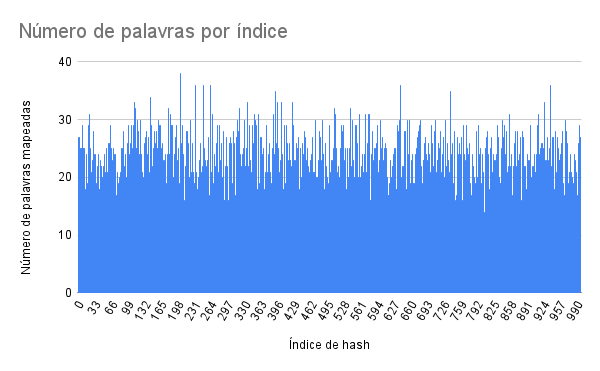
\includegraphics[width=0.9\textwidth]{polinomial.png} % Nome do gráfico gerado
\caption{Distribuição de palavras distintas por índice da tabela usando a função de hash polinomial com base 31.}
\end{figure}

\subsubsection*{Por que essa função funciona melhor?}

Comparada à função da soma, a função polinomial apresenta várias vantagens:

\begin{itemize}
  \item \textbf{Considera a ordem dos caracteres:} isso evita que anagramas gerem o mesmo valor de hash.
  \item \textbf{Maior variação:} o uso de potências introduz um efeito de amplificação, mesmo para pequenas mudanças na string.
  \item \textbf{Distribuição mais equilibrada:} o número de posições ocupadas e a dispersão geral das chaves foram significativamente melhores.
\end{itemize}

Esse experimento mostra que, mesmo com um número de colisões inevitável quando $n \gg N$, uma função de hash bem projetada pode reduzir o impacto dessas colisões ao espalhar melhor os dados pela tabela.

\subsubsection*{Resultados com $N = 50000$}

Repetimos o experimento com a função polinomial base 31 utilizando uma tabela significativamente maior: $N = 50000$.

\begin{itemize}
  \item O número total de colisões foi de apenas \textbf{4.236};
  \item A maior carga observada em um único índice foi de \textbf{5 palavras distintas}.
\end{itemize}

Esses resultados mostram como o aumento do tamanho da tabela reduz drasticamente o número de colisões. 
Embora muitas posições da tabela fiquem vazias -- o que é natural quando $N$ é muito maior que o número de elementos -- as posições ocupadas recebem em geral apenas uma ou duas palavras. 
A distribuição resultante é bastante equilibrada, com poucas colisões e sem pontos de concentração.



\chapter{Resolução de Colisões}

Como vimos anteriormente, uma função de hash associa uma chave a uma posição em uma tabela, idealmente de forma uniforme e eficiente. 
No entanto, mesmo com boas funções de hash e tabelas com fator de carga controlado, colisões são inevitáveis: duas ou mais chaves diferentes podem ser mapeadas para o mesmo índice.

Essas colisões não indicam erro ou falha do algoritmo -- são uma consequência natural do mapeamento de um conjunto potencialmente muito grande de chaves em um espaço fixo de posições. 
A ocorrência de colisões exige que a implementação da tabela de dispersão adote estratégias específicas para resolvê-las. 
O objetivo destas estratégias é garantir que operações como inserção, busca e remoção continuem eficientes, mesmo quando múltiplas chaves disputam o mesmo espaço.

Neste capítulo, vamos estudar as principais abordagens para lidar com colisões: encadeamento ({\em chaining}), que utiliza listas para armazenar múltiplos elementos em uma mesma posição, e endereçamento aberto ({\em probing}), que busca novas posições disponíveis na própria tabela. 
Analisaremos o funcionamento de cada técnica, suas vantagens, limitações e os impactos que causam no desempenho da tabela.

\section{Encadeamento (Chaining)}

Uma das formas mais comuns de lidar com colisões em tabelas de dispersão é por meio do encadeamento. 
A ideia central dessa abordagem é permitir que múltiplos elementos ocupem a mesma posição da tabela, armazenando-os em uma estrutura auxiliar associada a cada índice -- geralmente, uma lista.

Em vez de restringir cada posição da tabela a conter no máximo um único elemento, o encadeamento permite que cada posição funcione como um ``balde'', onde várias chaves com o mesmo valor de hash podem ser inseridas. 
Assim, quando ocorre uma colisão, o novo elemento simplesmente é adicionado à lista existente naquele índice.

Por exemplo, se duas chaves diferentes forem mapeadas para a mesma posição pela função de hash, ambas serão armazenadas na lista associada àquela posição. 
A operação de busca percorre essa lista em busca da chave desejada; a inserção adiciona um novo elemento à lista; e a remoção procura pela chave e a elimina, se presente.

Essa abordagem é especialmente eficaz quando a função de hash distribui bem as chaves e o fator de carga da tabela permanece controlado. 
No entanto, se muitas colisões ocorrerem em um mesmo índice, a lista associada pode crescer, e o desempenho se degradar.

A seguir, veremos como essa estratégia é implementada e analisaremos seu impacto sobre o desempenho das operações básicas.

\subsection*{Estrutura de dados}

Na estratégia de encadeamento, cada posição da tabela de dispersão aponta para o início de uma lista ligada. 
Cada elemento dessa lista armazena um \textbf{par chave-valor}, além de um ponteiro para o próximo elemento.

Para isso, usamos duas estruturas em \texttt{C}:

\begin{lstlisting}[language=C, caption={Estrutura de um nó da lista encadeada}]
typedef struct No {
    char* chave;
    int valor;
    struct No* prox;
} No;
\end{lstlisting}

Essa estrutura representa um elemento armazenado em uma das listas. 
Ela contém:

\begin{itemize}
  \item \texttt{chave}: a chave do par (usamos \texttt{char*} para permitir chaves do tipo string),
  \item \texttt{valor}: o valor associado à chave (neste exemplo, um inteiro),
  \item \texttt{prox}: ponteiro para o próximo elemento da lista.
\end{itemize}

A tabela em si é representada por um vetor de ponteiros para \texttt{No}, encapsulado em uma estrutura \texttt{Dicionario}:

\begin{lstlisting}[language=C, caption={Estrutura do dicionário com tabela de dispersão}]
typedef struct {
    No* tabela[TAM];
} Dicionario;
\end{lstlisting}

Aqui, \texttt{TAM} é o tamanho da tabela (escolhido previamente). 
Cada entrada da tabela aponta para o início de uma lista de colisões -- ou é \texttt{NULL} se estiver vazia.

\subsection*{Função \texttt{criar}}

A função \texttt{criar} aloca dinamicamente uma estrutura do tipo \texttt{Dicionario} e inicializa todas as posições da tabela com o valor \texttt{NULL}, indicando que nenhuma chave foi inserida ainda. 
Cada posição da tabela está pronta para receber uma lista de colisões quando necessário.

\begin{lstlisting}[language=C, caption={Criação de um dicionário vazio}]
Dicionario* criar() {
    Dicionario* d = malloc(sizeof(Dicionario));
    for (int i = 0; i < TAM; i++)
        d->tabela[i] = NULL;
    return d;
}
\end{lstlisting}

Essa função:

\begin{itemize}
  \item Aloca memória para um novo dicionário;
  \item Inicializa todas as entradas da tabela com \texttt{NULL}, ou seja, listas vazias;
  \item Retorna um ponteiro para a estrutura recém-criada.
\end{itemize}

A tabela resultante está pronta para que as operações de inserção, remoção e busca sejam aplicadas. 
O tamanho da tabela, definido pela constante \texttt{TAM}, determina o número de ``baldes'' disponíveis para armazenar listas de colisões.

\subsection*{Função \texttt{inserir}}

A função \texttt{inserir(d, k, v)} insere o par \texttt{(k, v)} no dicionário \texttt{d}. 
Para isso, aplica a função de hash à chave \texttt{k} para determinar a posição na tabela, e então insere o par na lista ligada correspondente.

Se a chave \texttt{k} já estiver presente na lista, seu valor é atualizado.

\begin{lstlisting}[language=C, caption={Inserção de um par (k, v) na tabela}]
void inserir(Dicionario* d, const char* k, int v) {
    unsigned int h = hash(k);
    No* atual = d->tabela[h];

    while (atual != NULL) {
        if (strcmp(atual->chave, k) == 0) {
            atual->valor = v;  // substitui o valor existente
            return;
        }
        atual = atual->prox;
    }

    // cria novo nó e insere no início da lista
    No* novo = malloc(sizeof(No));
    novo->chave = strdup(k);
    novo->valor = v;
    novo->prox = d->tabela[h];
    d->tabela[h] = novo;
}
\end{lstlisting}

Essa função realiza os seguintes passos:

\begin{itemize}
  \item Aplica a função de hash à chave \texttt{k} para obter a posição \texttt{h} na tabela;
  \item Percorre a lista encadeada na posição \texttt{h} em busca de uma chave igual;
  \item Se encontrar, substitui o valor antigo por \texttt{v};
  \item Caso contrário, cria um novo nó e o insere no início da lista.
\end{itemize}

Inserir no início da lista é eficiente e não afeta a corretude, já que a ordem dos elementos na lista não é relevante para a tabela de dispersão.

\subsection*{Função \texttt{buscar}}

A função \texttt{buscar(d, k)} procura pela chave \texttt{k} no dicionário \texttt{d}. 
Aplica-se a função de hash à chave para localizar a lista correspondente e percorre-se essa lista à procura de um nó cuja chave seja igual a \texttt{k}. 
Se encontrado, retorna-se um ponteiro para o valor associado; caso contrário, retorna-se \texttt{NULL}.

\begin{lstlisting}[language=C, caption={Busca de uma chave na tabela}]
int* buscar(Dicionario* d, const char* k) {
    unsigned int h = hash(k);
    No* atual = d->tabela[h];

    while (atual != NULL) {
        if (strcmp(atual->chave, k) == 0)
            return &atual->valor;
        atual = atual->prox;
    }
    return NULL;
}
\end{lstlisting}

Essa função:

\begin{itemize}
  \item Aplica a função de hash à chave \texttt{k} para obter a posição \texttt{h};
  \item Percorre a lista encadeada na posição \texttt{h};
  \item Se encontrar um nó com chave igual a \texttt{k}, retorna o endereço do campo \texttt{valor};
  \item Se não encontrar, retorna \texttt{NULL}.
\end{itemize}

Como o valor retornado é um ponteiro, o usuário da função pode tanto ler quanto modificar diretamente o valor associado à chave.

\subsection*{Função \texttt{remover}}

A função \texttt{remover(d, k)} remove do dicionário \texttt{d} o par cuja chave é \texttt{k}, caso ele exista. Para isso, aplica-se a função de hash à chave para localizar a lista apropriada e percorre-se essa lista à procura do nó correspondente. Ao encontrar o nó, ele é retirado da lista e sua memória é liberada.

\begin{lstlisting}[language=C, caption={Remoção de uma chave da tabela}]
void remover(Dicionario* d, const char* k) {
    unsigned int h = hash(k);
    No* atual = d->tabela[h];
    No* anterior = NULL;

    while (atual != NULL) {
        if (strcmp(atual->chave, k) == 0) {
            if (anterior == NULL)
                d->tabela[h] = atual->prox;
            else
                anterior->prox = atual->prox;
            free(atual->chave);
            free(atual);
            return;
        }
        anterior = atual;
        atual = atual->prox;
    }
}
\end{lstlisting}

Essa função realiza os seguintes passos:

\begin{itemize}
  \item Aplica a função de hash à chave \texttt{k} para determinar a posição \texttt{h};
  \item Percorre a lista encadeada na posição \texttt{h}, mantendo um ponteiro para o nó atual e outro para o anterior;
  \item Se encontrar a chave, remove o nó da lista (ajustando os ponteiros) e libera a memória alocada para a chave e para o nó;
  \item Se a chave não for encontrada, a função não faz nada.
\end{itemize}

A presença do ponteiro \texttt{anterior} é essencial para que seja possível remover nós que não estejam na primeira posição da lista.

\section{Endereçamento Aberto (Probing)}

A segunda abordagem clássica para lidar com colisões em tabelas de dispersão é o \textbf{endereçamento aberto} (ou \textit{probing}). 
Diferentemente do encadeamento, onde cada posição da tabela pode armazenar uma lista de elementos, no endereçamento aberto toda a informação é armazenada diretamente no vetor da tabela, sem o uso de listas auxiliares.

Quando ocorre uma colisão -- isto é, quando a posição indicada pela função de hash já está ocupada -- o algoritmo busca uma \textbf{outra posição livre} dentro da própria tabela, de acordo com uma sequência determinada por uma regra de sondagem (o \textit{probe}).

A ideia é simples: em vez de manter múltiplos elementos por posição, o algoritmo tenta encontrar uma nova posição onde o par chave-valor possa ser inserido. 
Essa busca por uma nova posição segue uma ordem bem definida, que depende da técnica de probing utilizada (como sondagem linear, quadrática ou duplo hashing).

O mesmo procedimento é adotado para realizar buscas e remoções: a função de hash fornece a posição inicial, e a sequência de probing é seguida até encontrar a chave desejada ou uma posição vazia que indique sua ausência.

Essa estratégia evita a alocação dinâmica de memória e torna a estrutura mais compacta, mas depende de que a tabela tenha \textbf{espaço disponível}, ou seja, seu fator de carga deve ser mantido abaixo de um certo limite para garantir bom desempenho.

É importante observar que, no endereçamento aberto, o fator de carga da tabela deve ser estritamente menor que $1$. 
Como não há listas auxiliares, todos os elementos precisam estar contidos diretamente na tabela. 
Se a tabela estiver completamente cheia, não é possível inserir novos elementos, independentemente da estratégia de sondagem utilizada.

Essa restrição não existe no caso do encadeamento, onde cada posição da tabela pode armazenar múltiplos elementos por meio de listas. 
Lá, o fator de carga pode inclusive ultrapassar $1$ -- embora, nesse caso, o desempenho possa piorar progressivamente.

Por isso, ao utilizar probing, é fundamental manter o fator de carga sob controle -- muitas implementações realocam ({\em rehash}) a tabela automaticamente ao atingir, por exemplo, $70\%$ de ocupação.

A forma mais simples de sondagem é a chamada \textbf{sondagem linear} (\textit{linear probing}). 
Nesse método, ao detectar uma colisão na posição $h$, verifica-se sequencialmente as posições $h+1$, $h+2$, $h+3$, e assim por diante (com aritmética modular), até encontrar uma posição vazia ou a chave procurada. 
Essa estratégia é fácil de implementar e eficiente com fator de carga baixo, mas pode causar aglomeração de elementos (\textit{clustering}), o que degrada o desempenho das operações.

Além da sondagem linear, existem outras estratégias, como a \textbf{sondagem quadrática} e o \textbf{duplo hashing}, que serão apresentadas brevemente ao final desta seção.

\subsection*{Função \texttt{criar}}

A função \texttt{criar} aloca uma estrutura de tabela de dispersão usando endereçamento aberto com sondagem linear. 
Como não há listas auxiliares, a tabela é simplesmente um vetor de ponteiros para pares chave-valor. 
Cada posição começa como \texttt{NULL}, indicando que está livre.

A estrutura usada é levemente diferente da versão com encadeamento: agora, armazenamos diretamente os pares no vetor. Para isso, usamos a seguinte definição:

\begin{lstlisting}[language=C, caption={Estrutura do par chave-valor com marcador de ocupação}]
typedef struct {
    char* chave;
    int valor;
} Entrada;

typedef struct {
    Entrada* tabela[TAM];
} Dicionario;
\end{lstlisting}

Note que o vetor contém ponteiros para \texttt{Entrada}. 
Uma posição \texttt{NULL} indica que está livre. Para marcação de remoções (discutida depois), pode-se usar um valor especial (como um ponteiro constante) para distinguir entre posição nunca usada e posição já removida.

A função de criação inicializa todas as posições com \texttt{NULL}:

\begin{lstlisting}[language=C, caption={Criação de tabela com sondagem linear}]
Dicionario* criar() {
    Dicionario* d = malloc(sizeof(Dicionario));
    for (int i = 0; i < TAM; i++)
        d->tabela[i] = NULL;
    return d;
}
\end{lstlisting}

Essa estrutura prepara o dicionário para operar com sondagem linear: cada inserção buscará uma posição livre, e cada busca percorrerá posições sucessivas até encontrar a chave ou uma posição vazia.

\subsection*{Função \texttt{inserir}}

A função \texttt{inserir(d, k, v)} aplica a função de hash à chave \texttt{k} e, em caso de colisão, procura a próxima posição livre na tabela, avançando sequencialmente até encontrar uma posição disponível ou uma chave já existente (caso em que o valor é substituído).

\begin{lstlisting}[language=C, caption={Inserção com sondagem linear}]
void inserir(Dicionario* d, const char* k, int v) {
    unsigned int h = hash(k);
    for (int i = 0; i < TAM; i++) {
        int pos = (h + i) % TAM;
        Entrada* e = d->tabela[pos];

        if (e == NULL) {
            // posição livre: inserir nova entrada
            e = malloc(sizeof(Entrada));
            e->chave = strdup(k);
            e->valor = v;
            d->tabela[pos] = e;
            return;
        }

        if (strcmp(e->chave, k) == 0) {
            // chave já presente: substituir valor
            e->valor = v;
            return;
        }
    }

    // tabela cheia (fator de carga >= 1)
    printf("Erro: tabela cheia.\n");
}
\end{lstlisting}

Essa função:

\begin{itemize}
  \item Calcula a posição inicial com a função de hash;
  \item Verifica sequencialmente as posições seguintes (com aritmética modular);
  \item Insere o par na primeira posição livre encontrada;
  \item Se a chave já existir, substitui o valor antigo;
  \item Se nenhuma posição estiver livre, exibe uma mensagem de erro.
\end{itemize}

\subsection*{Função \texttt{buscar}}

A função \texttt{buscar(d, k)} procura pela chave \texttt{k} na tabela usando sondagem linear. 
A partir da posição fornecida pela função de hash, percorre-se sequencialmente a tabela até encontrar a chave ou até chegar a uma posição vazia -- o que indica que a chave não está presente.

\begin{lstlisting}[language=C, caption={Busca com sondagem linear}]
int* buscar(Dicionario* d, const char* k) {
    unsigned int h = hash(k);
    for (int i = 0; i < TAM; i++) {
        int pos = (h + i) % TAM;
        Entrada* e = d->tabela[pos];

        if (e == NULL)
            return NULL; // posição nunca usada: chave não está na tabela

        if (strcmp(e->chave, k) == 0)
            return &e->valor; // chave encontrada
    }

    return NULL; // chave não encontrada após varrer toda a tabela
}
\end{lstlisting}

Essa função:

\begin{itemize}
  \item Calcula a posição inicial com a função de hash;
  \item Percorre posições consecutivas, segundo a regra da sondagem linear;
  \item Interrompe se encontrar a chave procurada ou uma posição nunca usada;
  \item Retorna um ponteiro para o valor correspondente, ou \texttt{NULL} se a chave não for encontrada.
\end{itemize}

A verificação de posição vazia é essencial para determinar que a chave não está na tabela. 
Isso é possível porque posições nunca utilizadas são inicializadas como \texttt{NULL} na criação do dicionário.

\subsection*{Função \texttt{remover}}

A operação de remoção em tabelas com sondagem linear exige cuidado: ao remover uma entrada, \textbf{não podemos simplesmente colocar \texttt{NULL}} na posição, pois isso interromperia buscas por chaves que foram inseridas após uma colisão e deslocadas para posições seguintes.

Para contornar esse problema, usamos um marcador especial para indicar que a posição foi ocupada no passado mas está \textbf{atualmente removida}. 
Um valor comum para isso é um ponteiro constante, que nunca será confundido com uma entrada válida nem com \texttt{NULL}:

\begin{lstlisting}[language=C, caption={Marcador especial para posição removida}]
#define REMOVIDO ((Entrada*) -1)
\end{lstlisting}

Com isso, a função de remoção pode ser implementada da seguinte forma:

\begin{lstlisting}[language=C, caption={Remoção com sondagem linear}]
void remover(Dicionario* d, const char* k) {
    unsigned int h = hash(k);
    for (int i = 0; i < TAM; i++) {
        int pos = (h + i) % TAM;
        Entrada* e = d->tabela[pos];

        if (e == NULL)
            return; // posição nunca usada: chave não está na tabela

        if (e != REMOVIDO && strcmp(e->chave, k) == 0) {
            free(e->chave);
            free(e);
            d->tabela[pos] = REMOVIDO;
            return;
        }
    }
}
\end{lstlisting}

Essa função:

\begin{itemize}
  \item Aplica a função de hash à chave;
  \item Percorre a tabela segundo a sondagem linear;
  \item Se encontrar a chave, libera sua memória e marca a posição como \texttt{REMOVIDO};
  \item Se encontrar uma posição \texttt{NULL}, termina a busca (a chave não está presente).
\end{itemize}

Ao marcar a posição como \texttt{REMOVIDO}, mantemos o funcionamento correto das buscas futuras, que devem continuar além dessa posição ao procurar por chaves deslocadas por colisão.

Na prática, também é possível reaproveitar posições marcadas como \texttt{REMOVIDO} durante inserções -- o que melhora o uso do espaço --, mas essa otimização não está incluída aqui para manter o código simples.

\subsection*{Outras formas de sondagem}

A sondagem linear é simples e eficiente enquanto o fator de carga da tabela permanece baixo. 
No entanto, ela sofre de um problema conhecido como \textbf{clustering primário}. 
Esse fenômeno ocorre quando várias chaves colidem na mesma região da tabela e passam a ocupar posições consecutivas.

Como a sondagem linear sempre verifica posições adjacentes em caso de colisão, uma sequência de elementos tende a crescer como um bloco contínuo. 
Quando novas colisões ocorrem, é mais provável que elas aconteçam dentro desse bloco -- o que aumenta o número médio de tentativas necessárias para inserção e busca. 
Esse acúmulo progressivo de elementos em regiões contíguas da tabela pode degradar o desempenho da estrutura significativamente, mesmo quando a tabela ainda não está cheia.

Para reduzir esse efeito, foram propostas estratégias de sondagem que espalham melhor as colisões pela tabela. 
As duas mais conhecidas são a \textbf{sondagem quadrática} e o \textbf{duplo hashing}.

Na \textbf{sondagem quadrática}, as posições alternativas são calculadas com base em deslocamentos quadráticos em relação à posição original. 
Ou seja, se a função de hash retorna a posição $h$, as próximas posições a serem testadas são:

\[
h + 1^2, \quad h + 2^2, \quad h + 3^2, \quad \ldots
\]

Em termos práticos, a $i$-ésima tentativa verifica a posição $(h + i^2) \bmod m$, onde $m$ é o tamanho da tabela. 
Essa estratégia evita a formação de \textit{clusters} lineares como ocorre na sondagem linear, pois espaça mais as tentativas e distribui os elementos de maneira mais uniforme.

No entanto, a sondagem quadrática apresenta duas limitações importantes:

\begin{itemize}
  \item Nem sempre garante que todas as posições da tabela serão visitadas, o que pode impedir a inserção de novos elementos mesmo antes de a tabela estar completamente cheia.
  \item Requer que o tamanho da tabela obedeça a certas propriedades (como ser um número primo ou uma potência de dois com ajustes) para garantir boa cobertura.
\end{itemize}

O \textbf{duplo hashing} utiliza uma segunda função de hash para definir o deslocamento entre uma tentativa e outra. 
A sequência de posições testadas é dada por:

\[
h + i \cdot h_2(k) \bmod m
\]

onde $h$ é o valor da primeira função de hash, $h_2(k)$ é a segunda função de hash aplicada à chave $k$, e $i$ é o número da tentativa.

A principal vantagem do duplo hashing é a sua capacidade de distribuir as colisões de forma menos previsível e mais uniforme pela tabela, reduzindo significativamente o problema do \textit{clustering}. 
Além disso, com uma boa escolha da segunda função de hash (por exemplo, garantindo que ela nunca retorne zero), o método pode percorrer toda a tabela antes de repetir posições.

A desvantagem é que o cálculo da segunda função de hash pode aumentar o custo computacional das operações, além de exigir maior cuidado no projeto das funções para evitar ciclos ou repetições.

Essas técnicas são especialmente úteis quando se deseja melhorar o desempenho de tabelas com fator de carga mais alto, desde que a tabela seja redimensionada adequadamente antes de atingir a saturação.

\subsection*{Clustering}

Para ilustrar o problema do \textit{clustering} e comparar as estratégias de sondagem, realizamos um experimento empírico utilizando as palavras distintas extraídas do livro \textit{O Arquipélago Gulag}, de Aleksandr Soljenítsin. 
O total de palavras distintas foi de 22.077, e elas foram inseridas em uma tabela de dispersão de tamanho $m = 50.000$ utilizando três métodos distintos: sondagem linear, sondagem quadrática e duplo hashing.

Usamos a função de hash polinomial com base 31 para calcular a posição inicial de cada palavra. 
No caso do duplo hashing, uma segunda função de hash foi obtida aplicando novamente a função polinomial à chave original.

Após a inserção de todas as palavras, analisamos a distribuição das posições ocupadas na tabela. 
Em particular, medimos o número de blocos consecutivos de posições ocupadas com comprimento superior a certos limiares (10, 20, 30, 40 e 50 posições). 
Os resultados obtidos estão resumidos na tabela a seguir:

\begin{center}
\begin{tabular}{lrrrrr}
\hline
\textbf{Método} & \textbf{$>$10} & \textbf{$>$20} & \textbf{$>$30} & \textbf{$>$40} & \textbf{$>$50} \\
\hline
Sondagem Linear      & 140 & 41 & 18 & 12 & 8 \\
Sondagem Quadrática  & 138 & 27 & 7  & 6  & 4 \\
Duplo Hashing        &  85 &  3 & 0  & 0  & 0 \\
\hline
\end{tabular}
\end{center}

Os resultados demonstram de forma clara o impacto do \textit{clustering primário} na sondagem linear. 
Mesmo com fator de carga abaixo de 50\%, esse método produziu diversos blocos com mais de 50 posições consecutivas ocupadas, tornando a tabela densamente preenchida em certas regiões.

A sondagem quadrática melhora essa situação, reduzindo significativamente o número de blocos longos, embora ainda apresente alguma aglomeração local. 
Já o duplo hashing praticamente elimina o fenômeno: não se observa nenhum bloco com mais de 30 posições consecutivas ocupadas, indicando uma distribuição muito mais uniforme e eficiente.

A estratégia adotada para lidar com colisões varia entre linguagens de programação e suas bibliotecas padrão. 
No caso da linguagem \textbf{Java}, a classe \texttt{HashMap} utiliza por padrão a técnica de \textbf{encadeamento} (\textit{chaining}), armazenando listas de pares chave-valor em cada posição da tabela. 
Desde o Java 8, quando uma lista encadeada cresce além de um certo limite (por padrão, 8 elementos), ela é automaticamente convertida em uma árvore balanceada (veremos isso nos capítulos adjacentes), melhorando o desempenho no pior caso\footnote{\url{https://www.javapedia.net/Map-and-its-implementations/2606}}. 

Em contraste, a linguagem \textbf{Python} implementa seus dicionários (\texttt{dict}) e conjuntos (\texttt{set}) com base em \textbf{endereçamento aberto} (\textit{open addressing}), resolvendo colisões por meio de \textbf{sondagem linear modificada}. 
A partir da versão 3.6, os dicionários passaram a preservar a ordem de inserção dos pares chave-valor, sem alterar o mecanismo fundamental de resolução de colisões.

A implementação do \texttt{dict} em CPython utiliza deslocamentos calculados a partir do hash da chave, com ajustes dinâmicos e política de inserção que favorece a ocupação de posições mais próximas à posição ideal. 
Essa abordagem é inspirada em técnicas como o \textit{robin hood hashing}, nas quais elementos com maior ``idade de inserção'' podem ser mantidos em posições melhores em detrimento de elementos mais recentes. 
Essa estratégia melhora a distribuição das colisões, reduz o \textit{clustering} primário e favorece a localidade de memória, contribuindo para o desempenho eficiente mesmo sob fatores de carga elevados.

\chapter{Análise de Desempenho dos Métodos de Hash}

Neste capítulo, analisaremos o desempenho das principais estratégias de implementação de tabelas de dispersão, com ênfase nas operações de inserção e busca. 
Consideraremos tanto o \textbf{pior caso} quanto o \textbf{caso médio}, comparando os métodos de encadeamento e de endereçamento aberto sob diferentes condições de uso.

A análise será feita utilizando a \textbf{notação assintótica} $\Theta$, que descreve a ordem de crescimento do tempo de execução das operações em função do número de elementos armazenados. 
Quando dizemos que uma operação tem custo $\Theta(n)$, queremos dizer que o tempo de execução cresce proporcionalmente a $n$, tanto como limite superior quanto inferior. 
De forma análoga, $\Theta(1)$ indica que o tempo de execução permanece constante, independentemente do tamanho da entrada.

\begin{center}
\noindent\fbox{%
    \parbox{0.95\textwidth}{%
        \textbf{Hipótese da função de hash uniforme:} Para todas as análises de caso médio apresentadas neste capítulo, assumiremos que a função de hash utilizada distribui as chaves de forma \textbf{uniforme} e \textbf{aleatória} entre as posições da tabela. 
    }
}
\end{center}

Seja $n$ o número total de elementos armazenados na tabela e $m$ o tamanho da tabela (isto é, o número de posições disponíveis). 
O \textbf{fator de carga} é definido por:

\[
\alpha = \frac{n}{m}
\]

Esse fator expressa a média de elementos por posição da tabela. 
No caso de encadeamento, representa o comprimento médio das listas associadas a cada posição. 
No caso de endereçamento aberto, indica a proporção da tabela que está ocupada.

\section{Encadeamento}

No encadeamento, cada posição da tabela aponta para uma lista encadeada contendo os pares chave–valor cujas chaves foram mapeadas para aquela posição pela função de hash. Essa abordagem é simples, flexível e lida bem com colisões, desde que o fator de carga seja mantido sob controle.

\subsection*{Custo de busca}

A seguir, analisamos o custo da operação de busca, tanto no caso médio quanto no pior caso. 
Para essa análise, usamos a notação $\Theta$ para indicar a ordem exata de crescimento do tempo de execução em função do número de elementos armazenados.

Sob a hipótese de que a função de hash distribui as chaves uniformemente entre as $m$ posições da tabela, temos:

\begin{itemize}
  \item \textbf{Busca bem-sucedida:} a chave está presente e espera-se que esteja distribuída uniformemente. 
  Nesse caso, o custo médio é
  \[
  \Theta\left(1 + \frac{\alpha}{2}\right)
  \]
  pois percorremos, em média, metade da lista associada à posição. 
  Em particular, se garantimos que $n = O(m)$, ou seja, o número de elementos cresce no máximo linearmente com o tamanho da tabela, o custo médio torna-se
  \[
  \Theta(1)
  \]

  \item \textbf{Busca mal-sucedida:} a chave não está presente e percorremos toda a lista daquela posição para verificar sua ausência. 
  O custo médio é
  \[
  \Theta(\alpha)
  \]
\end{itemize}

No pior caso, todas as $n$ chaves colidem na mesma posição da tabela, formando uma única lista encadeada. 
A busca, nesse cenário, precisa percorrer a lista inteira:

\[
\Theta(n)
\]

\subsection{Custo de inserção}

A inserção em tabelas com encadeamento consiste em adicionar um novo par chave–valor na lista associada à posição calculada pela função de hash. 
Se a chave já estiver presente, o valor é atualizado; caso contrário, um novo nó é adicionado.

Assumindo novamente uma distribuição uniforme das chaves, espera-se que o comprimento médio de cada lista seja proporcional ao fator de carga~$\alpha$. 
Como a inserção é realizada no início da lista (sem necessidade de percorrê-la), o custo da operação é constante:

\[
\Theta(1)
\]

No pior caso, todas as chaves colidem na mesma posição da tabela, formando uma única lista encadeada de comprimento~$n$. 
Se for necessário verificar a existência prévia da chave antes de inserir (como em um dicionário), é preciso percorrer toda a lista. 
O custo, portanto, é:

\[
\Theta(n)
\]

\section{Endereçamento Aberto}

No endereçamento aberto, todos os elementos são armazenados diretamente na tabela. 
Quando ocorre uma colisão, a função de hash é ajustada de forma sistemática para sondar outras posições disponíveis. 
Neste modelo, não há listas auxiliares: todas as chaves ocupam posições dentro do vetor principal.

No \emph{linear probing}, em caso de colisão, procuramos sequencialmente pela próxima posição livre na tabela. 

\subsection*{Caso médio}

Assumindo que as chaves são distribuídas de forma uniforme e aleatória e que a tabela ainda não está muito cheia (isto é, $\alpha < 1$), temos os seguintes custos médios para busca no \emph{linear probing}, conforme a análise clássica de Knuth\footnote{Donald E. Knuth. \textit{The Art of Computer Programming}, Volume 3: \textit{Sorting and Searching}, 2nd ed., Addison-Wesley, 1998. Seção 6.4.}:

\begin{itemize}
  \item \textbf{Busca mal-sucedida:}
  \[
  \Theta\left( \frac{1}{2} \left(1 + \frac{1}{(1 - \alpha)^2} \right) \right)
  \]

  \item \textbf{Busca bem-sucedida:}
  \[
  \Theta\left( \frac{1}{2} \left(1 + \frac{1}{1 - \alpha} \right) \right)
  \]
\end{itemize}

Não desenvolveremos aqui a demonstração dessas expressões, mas elas ilustram como o custo médio de busca cresce rapidamente à medida que o fator de carga $\alpha$ se aproxima de 1. 
Em particular, o desempenho se mantém eficiente apenas enquanto $\alpha$ for significativamente menor do que 1.

\section{Comparação dos métodos}

As Tabelas a seguir resumem os custos médios e de pior caso das operações de busca e inserção nas principais estruturas discutidas. 
A lista ligada é apresentada como referência: embora tenha inserção eficiente no início da lista, sua busca é linear no número de elementos. 
O encadeamento oferece inserção rápida e desempenho de busca que depende do fator de carga~$\alpha = n/m$; quando esse fator é mantido constante, tanto a busca quanto a inserção apresentam custo constante no caso médio. 
No endereçamento aberto com sondagem linear, o custo médio das operações cresce rapidamente à medida que~$\alpha$ se aproxima de 1, conforme indicado pelas expressões assintóticas. 
Em todos os métodos, o pior caso pode chegar a~$\Theta(n)$, o que reforça a importância de uma boa função de hash e do controle rigoroso do fator de carga.

\begin{table}[h!]
\centering
\caption{Desempenho médio das operações}
\begin{tabular}{|l|c|c|}
\hline
\textbf{Estrutura} & \textbf{Busca (média)} & \textbf{Inserção (média)} \\
\hline
Lista ligada        & $\Theta(n)$ & $\Theta(1)$ \\
Encadeamento        & $\Theta(1 + \alpha)$ & $\Theta(1)$ \\
Sondagem linear     & $\Theta\left( \frac{1}{1 - \alpha} \right)$ & $\Theta\left( \frac{1}{1 - \alpha} \right)$ \\
\hline
\end{tabular}
\end{table}


\begin{table}[h!]
\centering
\caption{Desempenho no pior caso}
\begin{tabular}{|l|c|c|}
\hline
\textbf{Estrutura} & \textbf{Busca (pior)} & \textbf{Inserção (pior)} \\
\hline
Lista ligada        & $\Theta(n)$ & $\Theta(1)$ \\
Encadeamento        & $\Theta(n)$ & $\Theta(n)$ \\
Sondagem linear     & $\Theta(n)$ & $\Theta(n)$ \\
\hline
\end{tabular}
\end{table}

\chapter{Exercícios}

\begin{exercicio}
Considere uma tabela de dispersão com $m = 13$ posições e $n = 9$ elementos.
\begin{enumerate}
  \item Calcule o fator de carga $\alpha$.
  \item Supondo uso de encadeamento, qual é o comprimento médio das listas?
  \item O que aconteceria com $\alpha$ e com o desempenho das operações se inserirmos mais 10 elementos sem aumentar o tamanho da tabela?
\end{enumerate}
\end{exercicio}

\begin{exercicio}
Explique o papel da função de hash no desempenho das tabelas de dispersão.
\begin{enumerate}
  \item O que significa dizer que uma função de hash é “uniforme”?
  \item Dê um exemplo simples de função de hash não uniforme e explique por que ela pode causar degradação de desempenho.
  \item Qual a relação entre a qualidade da função de hash e o pior caso de busca?
\end{enumerate}
\end{exercicio}

\begin{exercicio}
Compare as estratégias de resolução de colisão.
\begin{enumerate}
  \item Descreva a diferença entre encadeamento e endereçamento aberto com sondagem linear.
  \item Por que o encadeamento é considerado mais robusto em cenários de alto fator de carga?
  \item O que é \emph{clustering primário} e como ele afeta a sondagem linear?
\end{enumerate}
\end{exercicio}

\begin{exercicio}
Considere um sistema com sondagem linear e fator de carga $\alpha = 0{,}75$.
\begin{enumerate}
  \item Estime o custo médio de uma busca bem-sucedida e uma mal-sucedida com base nas fórmulas de Knuth (não é necessário justificar a fórmula).
  \item E se $\alpha = 0{,}95$?
  \item Por que o controle de $\alpha$ é mais crítico em sondagem linear do que em encadeamento?
\end{enumerate}
\end{exercicio}

\begin{exercicio}
Analise os seguintes cenários de desempenho:
\begin{enumerate}
  \item Qual é o custo médio da busca bem-sucedida em encadeamento com $\alpha = 3$?
  \item Qual é o pior caso para busca usando qualquer método de dispersão?
  \item Explique como o uso de rehashing pode garantir que o custo médio de busca permaneça constante.
\end{enumerate}
\end{exercicio}



\part{Árvores de Busca}
\chapter{Árvores Binárias de Busca}

Uma \textbf{árvore binária} é uma estrutura de dados hierárquica em que cada elemento, chamado de \emph{nó}, possui no máximo dois filhos: um à esquerda e outro à direita. 
Como nas tabelas de dispersão, cada nó pode conter uma chave (e eventualmente um valor associado), além de ponteiros para seus filhos esquerdo e direito. 
A estrutura é naturalmente recursiva: cada subárvore também é uma árvore binária.

As chaves em uma ABB devem ser \textbf{comparáveis} -- ou seja, é necessário poder determinar se uma chave é menor, igual ou maior que outra. 
Essa exigência é fundamental porque a estrutura da ABB depende de comparações para decidir a posição de cada chave.

\begin{center}
\noindent\fbox{%
    \parbox{0.95\textwidth}{%
        \textbf{Propriedade fundamental das ABBs:} Para cada nó com chave $k$, todas as chaves da \emph{subárvore esquerda} devem ser \emph{estritamente menores} que $k$, e todas as chaves da \emph{subárvore direita} devem ser \emph{estritamente maiores} que $k$.
    }
}
\end{center}


Essa organização garante que um percurso em ordem (esquerda $\rightarrow$ raiz $\rightarrow$ direita) produza as chaves em ordem crescente, o que permite a implementação eficiente de operações como busca, inserção, remoção e iteração ordenada.
 O fato de que as chaves são comparáveis torna possível usar ABBs para implementar um dicionário ordenado, em que é possível não apenas recuperar valores associados a chaves específicas, mas também navegar pelas chaves em ordem, encontrar o menor ou maior elemento, ou consultar faixas de valores.


As ABBs são utilizadas em contextos onde a ordenação é importante ou onde há necessidade de navegação eficiente por faixas de valores. Exemplos comuns incluem:

\begin{itemize}
  \item Implementação de \textbf{dicionários ordenados}
  \item Sistemas de \textbf{banco de dados} que requerem ordenação ou busca por intervalo
  \item \textbf{Sistemas de arquivos}, para indexação de nomes ou blocos
  \item Estruturas auxiliares em algoritmos de compressão, compiladores e engines de jogos
\end{itemize}

\section{Estrutura}

Uma árvore binária de busca é composta por nós que armazenam três informações principais:

\begin{itemize}
  \item uma \textbf{chave}, usada para determinar a posição do nó na árvore com base em comparações;
  \item um \textbf{valor} associado à chave, como em um dicionário;
  \item dois ponteiros, para os \textbf{filhos esquerdo e direito}.
\end{itemize}

Em C, essa estrutura pode ser representada por um \texttt{struct} da seguinte forma:

\begin{lstlisting}[language=C, caption={Estrutura de um nó de ABB}]
typedef struct no {
    int chave;
    void* valor;
    struct no* esq;
    struct no* dir;
} No;
\end{lstlisting}

O campo \texttt{chave} é usado para comparações, o campo \texttt{valor} pode apontar para qualquer tipo de dado associado, e os campos \texttt{esq} e \texttt{dir} representam, respectivamente, os filhos à esquerda e à direita do nó.

O ponteiro para a raiz da árvore representa a ABB como um todo. 
Todas as operações -- como busca, inserção e remoção -- são executadas a partir desse ponteiro, percorrendo a árvore com base na comparação das chaves.

Essa estrutura recursiva permite representar árvores de qualquer tamanho, e sua organização garante que operações fundamentais possam ser implementadas de forma eficiente.

\section{Função {\tt buscar}}

Dada uma árvore binária de busca e uma chave, a operação de \texttt{buscar} percorre a árvore a partir da raiz comparando a chave desejada com a chave do nó atual:

\begin{itemize}
  \item Se a chave for igual à do nó atual, o valor associado é retornado.
  \item Se for menor, a busca continua na subárvore esquerda.
  \item Se for maior, a busca continua na subárvore direita.
\end{itemize}

A seguir apresentamos a \textbf{versão recursiva} do algoritmo. 
Também é possível implementar a operação de forma iterativa, com uma estrutura de repetição.

\begin{lstlisting}[language=C, caption={Busca recursiva em ABB}]
void* buscar(No* raiz, int chave) {
    if (raiz == NULL)
        return NULL;
    if (chave == raiz->chave)
        return raiz->valor;
    if (chave < raiz->chave)
        return buscar(raiz->esq, chave);
    else
        return buscar(raiz->dir, chave);
}
\end{lstlisting}


O tempo de execução da operação de busca em uma árvore binária de busca é proporcional à altura da árvore. 
Em outras palavras, a busca sempre toma tempo $\Theta(h)$, onde $h$ representa a \textbf{altura da árvore}.

A altura de uma árvore é definida como o número de arestas no caminho mais longo entre a raiz e uma folha. 
Em uma árvore com apenas um único nó (a raiz), a altura é zero. 
Se a árvore tem dois níveis, com a raiz e dois filhos diretos, sua altura é 1. 
Intuitivamente, quanto mais ``profunda'' for a árvore, maior será a quantidade de comparações necessárias em uma busca.

No \textbf{pior caso}, a altura $h$ pode ser igual a $n - 1$, quando a árvore está completamente desbalanceada -- por exemplo, quando todas as chaves são inseridas em ordem crescente ou decrescente. 
Nessa situação, a árvore degenera em uma lista encadeada, e a busca tem complexidade $\Theta(n)$.

No \textbf{caso médio}, assumimos -- para fins de análise teórica - que as chaves são inseridas em ordem aleatória e com distribuição aproximadamente uniforme. 
Sob essa hipótese, a árvore resultante tende a ficar razoavelmente equilibrada.

Em uma árvore binária perfeitamente equilibrada, cada nível da árvore contém o dobro de nós do nível anterior:
\begin{itemize}
  \item nível $0$ (a raiz): $1$ nó
  \item nível $1$: até $2$ nós
  \item nível $2$: até $4$ nós
  \item nível $3$: até $8$ nós
  \item \dots
  \item nível $h$: até $2^h$ nós
\end{itemize}

Se somarmos o número total de nós da árvore até o nível $h$, temos:
\[
1 + 2 + 4 + \dots + 2^h = 2^{h+1} - 1
\]

Isso significa que uma árvore com altura $h$ pode conter até $2^{h+1} - 1$ nós. 
Invertendo essa relação, o número de níveis necessário para acomodar $n$ nós é aproximadamente $\log_2 n$. 
Assim, dizemos que uma árvore binária bem equilibrada tem altura $h = \Theta(\lg n)$.

Ou seja, se assumirmos que a ordem de iserção de chaves em um ABB foi feita de maneira aleatória -- algo difícil de garantir na prática -- sua altura é $\Theta(lg(n))$ e, consequentemente, a operação de busca é $\Theta(lg(n))$.

Portanto, embora a análise do caso médio sob inserção aleatória nos leve a uma altura logarítmica, essa não é uma suposição realista para aplicações em que os dados têm estrutura ou ordenação previsível. 
Nessas situações, o desempenho pode se degradar para o pior caso, com altura $\Theta(n)$. 
Para garantir bom desempenho independentemente da ordem de inserção, é necessário usar árvores com balanceamento automático que veremos mais a frente na apostila.


\section{Função \texttt{inserir}}

A operação de inserção em uma árvore binária de busca segue a mesma lógica da busca: percorremos a árvore comparando a nova chave com as chaves já presentes, até encontrar uma posição vazia (isto é, um ponteiro nulo) onde o novo nó deve ser inserido.

Se a chave já existe na árvore, podemos optar por atualizar o valor associado. 
Caso contrário, criamos um novo nó com a chave e o valor fornecidos, e o inserimos como filho de um nó existente.

A seguir apresentamos a versão recursiva da inserção:

\begin{lstlisting}[language=C, caption={Inserção recursiva em ABB}]
No* inserir(No* raiz, int chave, void* valor) {
    if (raiz == NULL) {
        No* novo = malloc(sizeof(No));
        novo->chave = chave;
        novo->valor = valor;
        novo->esq = NULL;
        novo->dir = NULL;
        return novo;
    }

    if (chave == raiz->chave)
        raiz->valor = valor; // atualiza
    else if (chave < raiz->chave)
        raiz->esq = inserir(raiz->esq, chave, valor);
    else
        raiz->dir = inserir(raiz->dir, chave, valor);

    return raiz;
}
\end{lstlisting}

Assim como na busca, a complexidade da inserção depende da altura da árvore. 
Em geral, a operação percorre o caminho da raiz até uma folha, realizando comparações até encontrar a posição correta.

\section{Função \texttt{remover}}

A operação de remoção em uma árvore binária de busca é mais complexa do que busca ou inserção, pois precisamos manter a propriedade de ordenação da árvore mesmo após retirar um nó.

Dado um nó a ser removido, três situações podem ocorrer:

\begin{enumerate}
  \item O nó não tem filhos: basta removê-lo.
  \item O nó tem apenas um filho: removemos o nó e conectamos seu filho diretamente ao pai.
  \item O nó tem dois filhos: substituímos o conteúdo do nó pela menor chave da subárvore direita (ou, alternativamente, pela maior da subárvore esquerda), e então removemos essa chave auxiliar da subárvore correspondente.
\end{enumerate}

A seguir mostramos uma implementação recursiva usando o menor elemento da subárvore direita como substituto:

\begin{lstlisting}[language=C, caption={Remoção recursiva em ABB}]
No* remover(No* raiz, int chave) {
    if (raiz == NULL)
        return NULL;

    if (chave < raiz->chave)
        raiz->esq = remover(raiz->esq, chave);
    else if (chave > raiz->chave)
        raiz->dir = remover(raiz->dir, chave);
    else {
        // caso 1 e 2: zero ou um filho
        if (raiz->esq == NULL) {
            No* temp = raiz->dir;
            free(raiz);
            return temp;
        }
        if (raiz->dir == NULL) {
            No* temp = raiz->esq;
            free(raiz);
            return temp;
        }

        // caso 3: dois filhos
        No* sucessor = raiz->dir;
        while (sucessor->esq != NULL)
            sucessor = sucessor->esq;

        raiz->chave = sucessor->chave;
        raiz->valor = sucessor->valor;
        raiz->dir = remover(raiz->dir, sucessor->chave);
    }

    return raiz;
}
\end{lstlisting}

Vale destacar que, embora a remoção envolva lógica mais elaborada, seu custo assintótico é o mesmo das demais operações: ele depende unicamente da altura da árvore.

\section{Menor e maior chave}

Em um dicionário ordenado implementado com uma árvore binária de busca, é comum precisar encontrar a menor ou a maior chave presente na estrutura. 
Essas operações são diretas graças à propriedade fundamental da ABB.

\textbf{Menor chave:} a menor chave está no nó mais à esquerda da árvore. 
Basta seguir os ponteiros para o filho esquerdo até encontrar um nó que não tenha filho à esquerda.

\textbf{Maior chave:} a maior chave está no nó mais à direita da árvore. 
O procedimento é simétrico ao anterior: seguimos os ponteiros para o filho direito até encontrar um nó sem filho à direita.

\begin{lstlisting}[language=C, caption={Busca da menor chave em ABB}]
No* minimo(No* raiz) {
    if (raiz == NULL)
        return NULL;
    while (raiz->esq != NULL)
        raiz = raiz->esq;
    return raiz;
}
\end{lstlisting}

\begin{lstlisting}[language=C, caption={Busca da maior chave em ABB}]
No* maximo(No* raiz) {
    if (raiz == NULL)
        return NULL;
    while (raiz->dir != NULL)
        raiz = raiz->dir;
    return raiz;
}
\end{lstlisting}

Essas operações percorrem apenas um caminho da raiz até uma folha, o que leva tempo $\Theta(h)$, onde $h$ é a altura da árvore. 

\section{Anterior e posterior}

Em um dicionário ordenado, é útil localizar a chave imediatamente anterior ou posterior a uma dada chave. 
Essas operações são chamadas de \textbf{predecessor} (anterior) e \textbf{sucessor} (posterior).

Dado um nó com chave $k$, temos duas situações para cada uma dessas operações:

\textbf{Anterior (predecessor):}

\begin{itemize}
  \item Se o nó tem subárvore esquerda, o predecessor é o maior nó dessa subárvore (ou seja, o mais à direita da subárvore esquerda).
  \item Se o nó não tem subárvore esquerda, o predecessor está entre os ancestrais: é o último ancestral pelo qual passamos \textbf{descendo para a direita}.
\end{itemize}

\textbf{Posterior (sucessor):}

\begin{itemize}
  \item Se o nó tem subárvore direita, o sucessor é o menor nó dessa subárvore (isto é, o mais à esquerda da subárvore direita).
  \item Se o nó não tem subárvore direita, o sucessor está entre os ancestrais: é o último ancestral pelo qual passamos \textbf{descendo para a esquerda}.
\end{itemize}

\textbf{Observação:} essas operações dependem do acesso direto ao nó cuja chave $k$ queremos usar como referência. 
Se partimos apenas da raiz e conhecemos a chave $k$, precisamos primeiro localizar o nó correspondente com uma busca.

A seguir, apresentamos uma versão recursiva que, a partir da raiz da árvore e de uma chave $k$, encontra o sucessor (posterior):

\begin{lstlisting}[language=C, caption={Busca do sucessor em ABB}]
No* sucessor(No* raiz, int chave) {
    No* atual = raiz;
    No* candidato = NULL;

    while (atual != NULL) {
        if (chave < atual->chave) {
            candidato = atual;
            atual = atual->esq;
        } else {
            atual = atual->dir;
        }
    }

    return candidato;
}
\end{lstlisting}

O algoritmo para o \texttt{predecessor} é análogo, trocando a lógica de comparação e os lados esquerdo/direito.

Como todas as operações anteriores, essas operações percorrem um único caminho da raiz até uma folha, tomando tempo $\Theta(h)$, onde $h$ é a altura da árvore. 


\section{Visita em ordem}

Uma das principais vantagens de usar uma árvore binária de busca é que ela permite percorrer todas as chaves em ordem crescente de maneira simples e eficiente.

O \textbf{percurso em ordem} (ou \emph{in-order traversal}) segue o seguinte padrão recursivo:

\begin{enumerate}
  \item Visita a subárvore esquerda;
  \item Visita o nó atual;
  \item Visita a subárvore direita.
\end{enumerate}

Esse padrão garante que as chaves sejam visitadas em ordem crescente, respeitando a propriedade estrutural da árvore binária de busca.

A seguir, apresentamos uma função que percorre a árvore e aplica uma função passada como parâmetro a cada chave e valor:

\begin{lstlisting}[language=C, caption={Percurso em ordem em ABB}]
void visitar_em_ordem(No* raiz, void (*visitar)(int, void*)) {
    if (raiz == NULL)
        return;

    visitar_em_ordem(raiz->esq, visitar);
    visitar(raiz->chave, raiz->valor);
    visitar_em_ordem(raiz->dir, visitar);
}
\end{lstlisting}

Essa função é útil para exibir os elementos do dicionário ordenado, salvar os pares chave-valor em um vetor, ou realizar qualquer outra operação sequencial.

A visita percorre todos os nós da árvore exatamente uma vez. 
Assim, sua complexidade é sempre $\Theta(n)$, independentemente da forma da árvore. 

\chapter{Árvores AVL}

Árvores binárias de busca (ABBs) são estruturas eficientes para armazenar dados ordenados, permitindo operações como busca, inserção e remoção em tempo proporcional à altura da árvore. 
Quando essa altura é pequena -- idealmente $\Theta(\lg(n))$ -- essas operações são rápidas. 
No entanto, a eficiência das ABBs depende diretamente de sua forma estrutural.

Em muitas situações práticas, a árvore pode crescer de forma desbalanceada. 
Isso ocorre, por exemplo, quando os dados são inseridos em ordem crescente ou decrescente -- casos extremos em que a ABB assume a forma de uma lista encadeada. 
Mas o problema não se limita a esses cenários: mesmo inserções em ordens menos regulares podem causar ramificações assimétricas, resultando em árvores com altura muito maior do que o necessário.

À medida que a altura cresce, o custo das operações também cresce. 
Uma ABB desbalanceada pode atingir altura linear no pior caso, tornando todas as operações proporcionalmente mais lentas -- de tempo logarítmico para tempo linear.

Para evitar essa degradação, surgem as chamadas \textit{árvores balanceadas}, que reorganizam sua estrutura a cada inserção ou remoção para manter a altura sob controle. O balanceamento visa preservar o desempenho logarítmico, limitando o crescimento desproporcional dos ramos. 
A árvore AVL, uma das primeiras estruturas desse tipo, impõe regras rígidas sobre o equilíbrio entre os ramos esquerdo e direito de cada nó, garantindo uma altura sempre próxima ao ideal.

Uma \textit{árvore AVL} é uma árvore binária de busca que mantém uma propriedade de balanceamento estrito: para todo nó da árvore, a diferença entre as alturas das subárvores esquerda e direita deve ser, no máximo, 1. 
Essa diferença é chamada de \textbf{fator de balanceamento} do nó.

Formalmente, seja $h_e$ a altura da subárvore esquerda de um nó e $h_d$ a altura da subárvore direita. 
A árvore é dita balanceada nesse nó se:

\[
|h_e - h_d| \leq 1
\]

Se essa condição for violada após uma operação de inserção ou remoção, a árvore executa uma ou mais rotações locais para restaurar o equilíbrio.

Esse critério local garante que a altura total da árvore permaneça $\Theta(\lg n)$, o que assegura que as operações de busca, inserção e remoção mantenham complexidade eficiente, mesmo no pior caso.

A estrutura foi proposta em 1962 pelos matemáticos soviéticos \textbf{Georgy Adelson-Velsky} e \textbf{Evgenii Landis}, cujos sobrenomes deram origem à sigla \textbf{AVL}. 
Foi a primeira árvore binária de busca com balanceamento automático proposta na literatura, e estabeleceu as bases para várias outras estruturas balanceadas utilizadas em algoritmos e sistemas de dados.

O \textbf{fator de balanceamento} de um nó em uma árvore AVL é definido como a diferença entre as alturas das subárvores esquerda e direita. 
Seja $h_e$ a altura da subárvore esquerda e $h_d$ a altura da subárvore direita de um nó. 
O fator de balanceamento $f$ é dado por:

\[
f = h_e - h_d
\]

Um nó está balanceado se $|f| \leq 1$. 
Se essa condição for violada após uma operação de inserção ou remoção -- isto é, se $f < -1$ ou $f > 1$ -- o nó está desbalanceado e a árvore precisa ser reestruturada.

O valor de $f$ é utilizado para determinar qual tipo de rotação é necessária para restaurar o equilíbrio da árvore. 
Os casos mais comuns são:

\begin{itemize}
    \item $f = 2$ e o fator do filho esquerdo $> 0$: rotação simples à direita.
    \item $f = 2$ e o fator do filho esquerdo $< 0$: rotação dupla esquerda-direita.
    \item $f = -2$ e o fator do filho direito $< 0$: rotação simples à esquerda.
    \item $f = -2$ e o fator do filho direito $> 0$: rotação dupla direita-esquerda.
\end{itemize}

Essas rotações locais garantem que a altura da árvore permaneça próxima de $\log n$, mesmo após modificações que causariam desequilíbrio.


\section{Rotações}

Quando uma inserção ou remoção causa desequilíbrio em um nó — isto é, quando $|h_e - h_d| > 1$ — a árvore AVL realiza rotações locais para restaurar o equilíbrio. As rotações ajustam a estrutura da árvore sem violar a propriedade de ordem da árvore binária de busca.

\subsection*{Rotação simples à direita}

Esse tipo de rotação é usado quando o desequilíbrio ocorre na subárvore esquerda de um nó, e essa subárvore também tem seu maior peso à esquerda. Isso ocorre, por exemplo, após a inserção em uma subárvore esquerda-esquerda.

\begin{center}
\begin{tikzpicture}[level distance=1.2cm,
  level 1/.style={sibling distance=3.5cm},
  level 2/.style={sibling distance=2cm}]

% Árvore antes
\node at (-5,0) {Antes da rotação:};

\node (A) at (-5,-1) {A}
  child {node (B) {B}
    child {node {C}}
    child [missing]
  }
  child [missing];

% seta
\draw[->, thick] (-2.5,-1) -- (-1.5,-1) node[midway, above] {rotação};

% Árvore depois
\node at (1,0) {Depois da rotação:};

\node (B2) at (1,-1) {B}
  child {node {C}}
  child {node (A2) {A}};

\end{tikzpicture}
\end{center}


\subsection*{Rotação simples à esquerda}

A rotação simples à esquerda é simétrica à rotação simples à direita, e ocorre quando o desequilíbrio está à direita de um nó, com o ramo mais pesado também à direita (caso direita-direita).

\begin{center}
\begin{tikzpicture}[level distance=1.2cm,
  level 1/.style={sibling distance=3.5cm},
  level 2/.style={sibling distance=2cm}]

% Árvore antes
\node at (-5,0) {Antes da rotação:};

\node (A) at (-5,-1) {A}
  child [missing]
  child {node (B) {B}
    child [missing]
    child {node {C}}
  };

% seta
\draw[->, thick] (-2.5,-1) -- (-1.5,-1) node[midway, above] {rotação};

% Árvore depois
\node at (1,0) {Depois da rotação:};

\node (B2) at (1,-1) {B}
  child {node (A2) {A}}
  child {node {C}};

\end{tikzpicture}
\end{center}

\subsection*{Rotação dupla esquerda-direita}

Esse tipo de rotação é necessário quando o desequilíbrio ocorre na subárvore esquerda de um nó, mas o maior peso está à direita dessa subárvore. É o caso típico após inserção em uma subárvore esquerda-direita. A correção envolve duas rotações: uma rotação simples à esquerda no filho esquerdo, seguida de uma rotação simples à direita no nó desbalanceado.

\begin{center}
\begin{tikzpicture}[level distance=1.2cm,
  level 1/.style={sibling distance=3.5cm},
  level 2/.style={sibling distance=2cm}]

% Árvore antes
\node at (-6,0) {Antes da rotação:};

\node (A) at (-6,-1) {A}
  child {node (B) {B}
    child [missing]
    child {node {C}}
  }
  child [missing];

% seta
\draw[->, thick] (-3,-1) -- (-2,-1) node[midway, above] {rotações};

% Árvore depois
\node at (2,0) {Depois da rotação:};

\node (C2) at (2,-1) {C}
  child {node (B2) {B}}
  child {node (A2) {A}};

\end{tikzpicture}
\end{center}


\subsection*{Rotação dupla direita-esquerda}

Esse tipo de rotação ocorre quando o desequilíbrio está na subárvore direita de um nó, mas o maior peso está à esquerda dessa subárvore. É o caso típico após inserção em uma subárvore direita-esquerda. A correção envolve duas rotações: uma rotação simples à direita no filho direito, seguida de uma rotação simples à esquerda no nó desbalanceado.

\begin{center}
\begin{tikzpicture}[level distance=1.2cm,
  level 1/.style={sibling distance=3.5cm},
  level 2/.style={sibling distance=2cm}]

% Árvore antes
\node at (-6,0) {Antes da rotação:};

\node (A) at (-6,-1) {A}
  child [missing]
  child {node (C) {C}
    child {node {B}}
    child [missing]
  };

% seta
\draw[->, thick] (-3,-1) -- (-2,-1) node[midway, above] {rotações};

% Árvore depois
\node at (2,0) {Depois da rotação:};

\node (B2) at (2,-1) {B}
  child {node (A2) {A}}
  child {node (C2) {C}};

\end{tikzpicture}
\end{center}

\section*{Função {\tt inserir}}

Antes de apresentar a inserção em uma árvore AVL, definimos três funções auxiliares essenciais para manter a propriedade de balanceamento da estrutura.

A função \texttt{altura} retorna a altura de um nó, considerando que um nó nulo tem altura $-1$:

\begin{lstlisting}
int altura(Node* n) {
    if (n == NULL)
        return -1;
    return n->altura;
}
\end{lstlisting}

A função \texttt{fatorBalanceamento} calcula a diferença entre as alturas das subárvores esquerda e direita de um nó:

\begin{lstlisting}
int fatorBalanceamento(Node* n) {
    if (n == NULL)
        return 0;
    return altura(n->esq) - altura(n->dir);
}
\end{lstlisting}

A função \texttt{max} retorna o maior entre dois inteiros:

\begin{lstlisting}
int max(int a, int b) {
    return (a > b) ? a : b;
}
\end{lstlisting}

A função \texttt{atualizarAltura} deve ser chamada sempre que a estrutura da árvore for modificada. 
Ela atualiza a altura de um nó com base nas alturas de seus filhos:

\begin{lstlisting}
void atualizarAltura(Node* n) {
    n->altura = 1 + max(altura(n->esq), altura(n->dir));
}
\end{lstlisting}

As rotações são operações locais que reestruturam a árvore para restaurar o balanceamento, mantendo a propriedade de ordem da árvore binária de busca.

\begin{lstlisting}
Node* rotacaoDireita(Node* y) {
    Node* x = y->esq;
    Node* T2 = x->dir;

    // Rotação
    x->dir = y;
    y->esq = T2;

    // Atualiza alturas
    atualizarAltura(y);
    atualizarAltura(x);

    return x;
}
\end{lstlisting}

\begin{lstlisting}
Node* rotacaoEsquerda(Node* x) {
    Node* y = x->dir;
    Node* T2 = y->esq;

    // Rotação
    y->esq = x;
    x->dir = T2;

    // Atualiza alturas
    atualizarAltura(x);
    atualizarAltura(y);

    return y;
}
\end{lstlisting}


A operação de inserção em uma árvore AVL segue o mesmo princípio da inserção em uma árvore binária de busca, mas com um passo adicional: após a inserção, é necessário verificar se houve desequilíbrio e aplicar rotações se necessário. 
A função abaixo insere uma nova chave e reequilibra a árvore:

\begin{lstlisting}
Node* inserir(Node* raiz, int chave) {
    if (raiz == NULL)
        return novoNo(chave);

    if (chave < raiz->chave)
        raiz->esq = inserir(raiz->esq, chave);
    else if (chave > raiz->chave)
        raiz->dir = inserir(raiz->dir, chave);
    else
        return raiz; // chaves duplicadas não são permitidas

    atualizarAltura(raiz);

    int fb = fatorBalanceamento(raiz);

    // Caso esquerda-esquerda
    if (fb > 1 && chave < raiz->esq->chave)
        return rotacaoDireita(raiz);

    // Caso direita-direita
    if (fb < -1 && chave > raiz->dir->chave)
        return rotacaoEsquerda(raiz);

    // Caso esquerda-direita
    if (fb > 1 && chave > raiz->esq->chave) {
        raiz->esq = rotacaoEsquerda(raiz->esq);
        return rotacaoDireita(raiz);
    }

    // Caso direita-esquerda
    if (fb < -1 && chave < raiz->dir->chave) {
        raiz->dir = rotacaoDireita(raiz->dir);
        return rotacaoEsquerda(raiz);
    }

    return raiz;
}
\end{lstlisting}

\section*{Função {\tt remover}}

A operação de remoção em uma árvore AVL começa como em uma árvore binária de busca: localiza-se o nó com a chave a ser removida, e aplica-se uma das três regras usuais:

\begin{itemize}
    \item Se o nó é uma folha, ele é simplesmente removido.
    \item Se tem apenas um filho, substitui-se o nó pelo filho.
    \item Se tem dois filhos, substitui-se o valor pela menor chave da subárvore direita (ou maior da esquerda), e remove-se esse sucessor recursivamente.
\end{itemize}

Após a remoção, a árvore pode ficar desbalanceada em vários nós no caminho de volta da recursão. 
Para cada nó, atualizamos a altura e aplicamos rotações se necessário.

\begin{lstlisting}
Node* remover(Node* raiz, int chave) {
    if (raiz == NULL)
        return NULL;

    if (chave < raiz->chave)
        raiz->esq = remover(raiz->esq, chave);
    else if (chave > raiz->chave)
        raiz->dir = remover(raiz->dir, chave);
    else {
        // Caso com 0 ou 1 filho
        if (raiz->esq == NULL || raiz->dir == NULL) {
            Node* temp = raiz->esq ? raiz->esq : raiz->dir;
            free(raiz);
            return temp;
        }

        // Caso com 2 filhos: substitui pelo menor da direita
        Node* temp = minimo(raiz->dir);
        raiz->chave = temp->chave;
        raiz->dir = remover(raiz->dir, temp->chave);
    }

    atualizarAltura(raiz);
    int fb = fatorBalanceamento(raiz);

    // Rebalanceamento

    // Caso esquerda-esquerda
    if (fb > 1 && fatorBalanceamento(raiz->esq) >= 0)
        return rotacaoDireita(raiz);

    // Caso esquerda-direita
    if (fb > 1 && fatorBalanceamento(raiz->esq) < 0) {
        raiz->esq = rotacaoEsquerda(raiz->esq);
        return rotacaoDireita(raiz);
    }

    // Caso direita-direita
    if (fb < -1 && fatorBalanceamento(raiz->dir) <= 0)
        return rotacaoEsquerda(raiz);

    // Caso direita-esquerda
    if (fb < -1 && fatorBalanceamento(raiz->dir) > 0) {
        raiz->dir = rotacaoDireita(raiz->dir);
        return rotacaoEsquerda(raiz);
    }

    return raiz;
}
\end{lstlisting}

A função \texttt{minimo} retorna o ponteiro para o nó com a menor chave em uma árvore, ou seja, o mais à esquerda.

\begin{lstlisting}
Node* minimo(Node* n) {
    while (n->esq != NULL)
        n = n->esq;
    return n;
}
\end{lstlisting}

Mesmo com o custo adicional de rotações, a remoção em uma árvore AVL continua com complexidade $O(\log n)$ no pior caso.

Como exemplo ilustrativo, considere a remoção do valor \texttt{10} em uma árvore AVL. 
O nó a ser removido possui dois filhos, o que exige que seja substituído por seu sucessor -- isto é, o menor elemento da subárvore direita, neste caso o nó \texttt{15}. 
Após a substituição, o nó \texttt{15} original é removido, e a árvore pode ficar desbalanceada, exigindo atualizações de altura e, se necessário, rotações. O diagrama a seguir mostra a árvore antes e depois da operação de remoção:

\begin{center}
\begin{tikzpicture}[level distance=1.2cm,
  level 1/.style={sibling distance=3.5cm},
  level 2/.style={sibling distance=2cm},
  every node/.style={font=\small}]

% Antes da remoção
\node at (-5,0) {Antes da remoção:};

\node (n10) at (-5,-1) {10}
  child {node {5}}
  child {node (n15) {15}
    child {node {12}}
    child {node {18}}
  };

% seta
\draw[->, thick] (-2,-1) -- (-1,-1) node[midway, above] {remoção};

% Depois da remoção
\node at (3,0) {Depois da remoção:};

\node (n15b) at (3,-1) {15}
  child {node {5}}
  child {node (n18) {18}
    child {node {12}}
    child [missing]
  };

\end{tikzpicture}
\end{center}


\section{Análise de Complexidade}

As árvores AVL mantêm a altura controlada por meio de um critério estrito de balanceamento, garantindo complexidade eficiente para todas as operações fundamentais.

Uma árvore AVL com $n$ nós tem altura $\Theta(\log n)$. 
Isso se deve ao fato de que, a cada nó, a diferença de altura entre as subárvores esquerda e direita é no máximo 1. 
Pode-se demonstrar, por indução, que a altura $h(n)$ de uma árvore AVL com $n$ nós satisfaz a desigualdade:

\[
h(n) \leq c \cdot \log_2(n + 1)
\]

para alguma constante $c$. 
Assim, as operações de busca, inserção e remoção têm complexidade assintótica proporcional à altura da árvore, isto é, $O(\log n)$.

As rotações são operações locais, que envolvem um número constante de atualizações de ponteiros e alturas. 
Cada rotação simples (à esquerda ou à direita) custa $O(1)$, e o mesmo vale para rotações duplas (compostas por duas rotações simples consecutivas). 
Assim, mesmo quando ocorrem, as rotações não aumentam a complexidade assintótica das operações principais.

A operação de inserção em uma árvore AVL realiza, no pior caso, um número proporcional a $\log n$ de chamadas recursivas, correspondente à altura da árvore. 
No entanto, o rebalanceamento necessário após a inserção afeta apenas o primeiro nó do caminho de volta cuja propriedade de balanceamento foi violada. 
Após aplicar a rotação apropriada nesse ponto -- seja simples ou dupla -- o equilíbrio é restaurado localmente, e os demais nós ancestrais não precisam de novas rotações, apenas de atualizações de altura.

Essa característica é uma consequência direta da estrutura da árvore AVL: como a inserção só aumenta a altura de uma subárvore em no máximo 1, e a rotação corrige esse crescimento excessivo, não é necessário propagar rotações por todo o caminho até a raiz. 
Portanto, embora o caminho de subida possa envolver até $O(\log n)$ atualizações de altura, apenas uma rotação (ou, no máximo, uma reestruturação composta por duas rotações simples) é realizada.

Assim, o custo total da inserção permanece $O(\log n)$ no pior caso, e o custo amortizado das rotações é constante.

A operação de remoção, no entanto, pode provocar desequilíbrios em múltiplos nós até a raiz. 
Ainda assim, o número total de rotações é limitado por $O(\log n)$, o que mantém o custo amortizado da remoção dentro da mesma ordem de complexidade.

\chapter{Árvores B}

Árvores B são estruturas de dados projetadas especificamente para contextos em que o custo do acesso à \textbf{memória externa} -- como discos rígidos ou SSDs -- é o principal gargalo de desempenho. 
Isso ocorre, por exemplo, em sistemas de arquivos, bancos de dados e outras aplicações que manipulam grandes volumes de dados que não cabem inteiramente na memória principal. 
Nesses casos, é essencial reduzir ao máximo a quantidade de acessos a disco, que são várias ordens de magnitude mais lentos do que os acessos à RAM.

Estruturas tradicionais como árvores binárias de busca balanceadas oferecem bom desempenho em memória, com altura proporcional a $\log n$, mas ainda exigem múltiplos acessos a diferentes blocos de disco: um para cada nível da árvore. 
Árvores B foram concebidas para esse cenário. 
Ao permitir que cada nó armazene várias chaves e tenha muitos filhos, elas reduzem a altura da árvore de $\log_2 n$ para $\log_t n$, com $t \gg 2$, o que diminui drasticamente o número de acessos à memória secundária necessários para localizar uma chave.

As \textbf{árvores B} são estruturas balanceadas que mantêm os dados ordenados e permitem operações eficientes de busca, inserção e remoção, mesmo em situações em que os dados estão distribuídos por centenas ou milhares de blocos de disco. 
Uma das características mais importantes dessas árvores é que cada nó pode conter várias chaves e ter múltiplos filhos, o que permite manter a altura da árvore pequena mesmo com um número muito grande de elementos.

Enquanto uma árvore binária de busca (ABB) tem no máximo dois filhos por nó e mantém uma única chave em cada nó, uma árvore B pode ter dezenas ou centenas de filhos por nó e armazenar múltiplas chaves. 
Isso permite que:
\begin{itemize}
\item A altura da árvore seja muito menor
\item A quantidade de acessos à memória externa seja reduzida
\item A inserção e remoção sejam feitas de forma eficiente mesmo em grandes volumes de dados
\end{itemize}

Além disso, ao contrário de árvores como as AVL, que focam em manter o tempo de operação em $O(\log n)$ com reestruturações locais, as árvores B são projetadas para alinhar sua estrutura à lógica de acesso por blocos, típica de discos e SSDs. 

A definição de uma árvore B depende de um parâmetro chamado \textit{grau mínimo}, denotado por $t$, com $t \geq 2$. 
Esse parâmetro determina os limites inferior e superior para o número de chaves que um nó pode armazenar. 
Cada nó da árvore (exceto a raiz) deve conter no mínimo $t - 1$ e no máximo $2t - 1$ chaves. 
Consequentemente, o número de filhos de um nó com $k$ chaves é $k + 1$, o que significa que cada nó interno pode ter entre $t$ e $2t$ filhos. 
A raiz é uma exceção: ela pode ter menos de $t - 1$ chaves (inclusive zero, no caso de uma árvore vazia).

As chaves em cada nó estão armazenadas em ordem crescente. 
Cada filho intercalado entre as chaves define um intervalo: o primeiro filho contém apenas chaves menores que a primeira chave do nó, o segundo filho contém chaves entre a primeira e a segunda chave, e assim por diante, até o último filho, que contém apenas chaves maiores que a última chave do nó.

Há dois tipos de nós em uma árvore B: os nós internos e as folhas. 
Os {\em nós internos} possuem filhos e organizam a estrutura da árvore; {\em as folhas}, por sua vez, não possuem filhos e armazenam apenas as chaves. 
Uma propriedade essencial das árvores B é que todas as folhas estão no mesmo nível, o que garante que a árvore seja perfeitamente balanceada -- todos os caminhos da raiz até as folhas têm o mesmo comprimento.

Essas regras garantem que a altura da árvore B cresça de forma lenta mesmo com um número muito grande de elementos. 
Como consequência, operações de busca, inserção e remoção mantêm complexidade logarítmica, mas com uma base maior no logaritmo, o que resulta em menos acessos a disco e melhor desempenho em sistemas com memória externa.

\section{Estrutura}

Cada nó em uma árvore B armazena um conjunto de chaves ordenadas e ponteiros para seus filhos. 
A estrutura de um nó com \( k \) chaves é composta por:

\begin{itemize}
  \item Um vetor de chaves ordenadas: \( k_1 < k_2 < \dots < k_k \)
  \item Um vetor de ponteiros para filhos: \( c_0, c_1, \dots, c_k \)
\end{itemize}

Cada ponteiro \( c_i \) aponta para uma subárvore que contém apenas chaves dentro de um intervalo bem definido:
\[
\text{Todas as chaves em } c_0 < k_1,\quad \text{todas as chaves em } c_1 \in (k_1, k_2),\quad \dots,\quad \text{todas em } c_k > k_k
\]

O número de filhos de um nó é sempre uma unidade a mais do que o número de chaves. 
Assim, um nó pode ter entre \( t - 1 \) e \( 2t - 1 \) chaves e entre \( t \) e \( 2t \) filhos (exceto a raiz).

\vspace{1em}
\textbf{Exemplo com \( t = 3 \):}

Neste caso, cada nó pode ter entre 2 e 5 chaves e entre 3 e 6 filhos. 
Abaixo está uma representação textual e visual de um nó que contém 3 chaves e, portanto, 4 filhos:
\vspace{1em}
Visualmente, esse nó pode ser representado assim:

\[
\begin{array}{cccccccccccc}
  \boxed{c_0}      &  k_1 = 17 & \boxed{c_1}       &  k_2 = 30 & \boxed{c_2}      &  k_3 = 42 & \boxed{c_3}        \\
   \downarrow      &           & \downarrow        &           & \downarrow       &           & \downarrow         \\
  \text{subárvore} &           & \text{subárvore}  &           & \text{subárvore} &           & \text{subárvore}
\end{array}
\]


Nesse exemplo, o nó possui três chaves ordenadas \( k_1 = 17 \), \( k_2 = 30 \), \( k_3 = 42 \), e quatro ponteiros \( c_0, c_1, c_2, c_3, c_4 \), intercalados entre as chaves. 
Cada ponteiro aponta para uma subárvore que cobre o intervalo correspondente:
\begin{itemize}
  \item \( c_0 \): chaves menores que 17
  \item \( c_1 \): chaves entre 17 e 30
  \item \( c_2 \): chaves entre 30 e 42
  \item \( c_3 \): chaves maiores que 42
\end{itemize}

Essa estrutura é especialmente eficiente para leitura em disco: o nó inteiro pode ser armazenado em um único bloco, e ao acessá-lo, o sistema já carrega diversas chaves e todos os ponteiros relevantes para decidir o próximo passo da busca, da inserção ou da remoção.

A seguir está o código em C que define a estrutura de uma árvore B com grau mínimo genérico \( t \), representado simbolicamente pela constante \texttt{T}. 
Cada nó pode armazenar até \( 2t - 1 \) chaves e até \( 2t \) ponteiros para filhos. 
No trecho abaixo, o valor de \texttt{T} está fixado em 3, mas ele pode ser ajustado conforme a aplicação.

\begin{lstlisting}
// Grau mínimo da árvore B
#define T 3

// Número máximo de chaves e filhos por nó
#define MAX_KEYS (2 * T - 1)
#define MAX_CHILDREN (2 * T)

// Estrutura de um nó da árvore B
typedef struct BTreeNode {
    int n;                           // Número de chaves atualmente no nó
    int is_leaf;                     // 1 se for folha, 0 caso contrário
    int keys[MAX_KEYS];             // Vetor de chaves ordenadas
    struct BTreeNode* children[MAX_CHILDREN];  // Ponteiros para os filhos
} BTreeNode;

// Estrutura da árvore B (mantém referência à raiz)
typedef struct BTree {
    BTreeNode* root;
} BTree;
\end{lstlisting}

A seguir, definimos funções para criar um novo nó e uma nova árvore B vazia com a raiz sendo uma folha:

\begin{lstlisting}
#include <stdlib.h>

// Cria um novo nó da árvore B
BTreeNode* create_node(int is_leaf) {
    BTreeNode* node = (BTreeNode*) malloc(sizeof(BTreeNode));
    node->n = 0;
    node->is_leaf = is_leaf;
    for (int i = 0; i < MAX_CHILDREN; i++) {
        node->children[i] = NULL;
    }
    return node;
}

// Cria uma nova árvore B com raiz vazia
BTree* create_btree() {
    BTree* tree = (BTree*) malloc(sizeof(BTree));
    tree->root = create_node(1);  // começa com a raiz sendo uma folha
    return tree;
}
\end{lstlisting}

\section{Função {\tt buscar}}

A operação de busca em uma árvore B segue o mesmo princípio das árvores de busca binária, porém adaptada para nós que contêm múltiplas chaves. A cada nível da árvore, a busca ocorre em dois passos:

\begin{enumerate}
  \item Percorremos sequencialmente o vetor de chaves do nó atual até encontrar a chave desejada ou uma chave maior.
  \item Se encontrarmos a chave, a busca termina com sucesso. 
  Caso contrário, seguimos para o filho correspondente, cujo intervalo contém a chave procurada.
\end{enumerate}

Como cada nó possui múltiplas chaves, conseguimos descartar grandes intervalos do espaço de busca em cada passo, mantendo a profundidade da árvore pequena (proporcional a \( \log_t n \)). 
Isso torna a busca eficiente, com poucos acessos a disco em aplicações de memória externa.

A busca é naturalmente recursiva, mas pode ser implementada iterativamente. 

\begin{lstlisting}
// Busca uma chave em um nó da árvore B (recursivamente)
BTreeNode* btree_search_node(BTreeNode* node, int key, int* index_out) {
    int i = 0;
    while (i < node->n && key > node->keys[i]) {
        i++;
    }

    if (i < node->n && key == node->keys[i]) {
        if (index_out) *index_out = i;
        return node;
    }

    if (node->is_leaf) return NULL;

    return btree_search_node(node->children[i], key, index_out);
}

// Busca uma chave na árvore B
BTreeNode* btree_search(BTree* tree, int key, int* index_out) {
    if (!tree || !tree->root) return NULL;
    return btree_search_node(tree->root, key, index_out);
}
\end{lstlisting}


A complexidade é \( O(\log n) \) no pior caso, tanto em número de comparações quanto em profundidade da árvore.

\section{Função {\tt inserir}}

O processo de inserção em árvores B mantém a árvore balanceada e todas as suas propriedades. 
O objetivo é inserir uma nova chave mantendo as chaves em ordem e garantindo que nenhum nó ultrapasse o número máximo de \( 2t - 1 \) chaves.

A inserção pode ocorrer em duas situações:

\begin{itemize}
  \item \textbf{Inserção em uma folha que ainda possui espaço:} a chave é inserida diretamente no vetor de chaves do nó, mantendo a ordenação.
  \item \textbf{Inserção em uma folha cheia:} o nó precisa ser dividido. A chave mediana sobe para o pai, e o nó é dividido em dois nós com \( t - 1 \) chaves cada.
\end{itemize}

Considere a inserção da chave 35 em um nó que já contém as chaves 17, 24, 30, 42 e 50. 
Com \( t = 3 \), o nó já está com o número máximo de chaves (\( 2t - 1 = 5 \)) e precisa ser dividido.

O processo é o seguinte:

\begin{enumerate}
  \item As chaves do nó são reorganizadas com a nova chave: 17, 24, 30, \textbf{35}, 42, 50.
  \item A chave mediana (35) é promovida ao nó pai.
  \item As chaves menores que 35 permanecem no nó original.
  \item As chaves maiores que 35 vão para um novo nó à direita.
\end{enumerate}

O diagrama abaixo mostra a estrutura antes e depois da divisão:

\vspace{1em}
\textbf{Antes da inserção:}
\[
\begin{array}{c}
\boxed{17 \quad 24 \quad 30 \quad 42 \quad 50}
\end{array}
\]

\textbf{Após tentativa de inserir 35 (antes da divisão):}
\[
\begin{array}{c}
\boxed{17 \quad 24 \quad 30 \quad \textbf{35} \quad 42 \quad 50}
\end{array}
\]

\textbf{Após a divisão:}
\[
\begin{array}{ccccccc}
  \boxed{c_i}                  &  k_1 = 35 & \boxed{c_{i+1}} \\
  \downarrow                   &           & \downarrow  \\
  \boxed{17 \quad 24 \quad 30} &           & \boxed{42 \quad 50}
\end{array}
\]

Se o nó pai também estiver cheio, o processo se repete recursivamente até (se necessário) a raiz ser dividida e a altura da árvore aumentar em 1.

Quando um nó folha está cheio e uma nova chave é inserida, ele é dividido e a chave mediana é promovida ao nó pai. 
Essa chave deve ser inserida em ordem no vetor de chaves do pai, e o novo ponteiro (referente ao nó criado à direita da divisão) deve ser inserido imediatamente à direita da nova chave.

Por exemplo, suponha que o nó pai inicialmente contenha:

\[
\begin{array}{ccccccc}
  \boxed{c_0}      &  k_1 = 12 & \boxed{c_1}                                    & k_2 = 55 & \boxed{c_2}     \\
  \downarrow       &           & \downarrow                                     &          & \downarrow      \\
  \text{subarvore} &           & \boxed{17 \quad 24 \quad 30 \quad 42 \quad 50} &          & \text{subarvore}
\end{array}
\]

Após a promoção da chave \( 35 \), ela deve ser inserida entre 12 e 55, e um novo ponteiro \( c_{\text{novo}} \) deve ser inserido à sua direita. O resultado será:

\[
\begin{array}{cccccccccc}
  \boxed{c_0}      &  k_1 = 12 & \boxed{c_1}                  & k_2 = 35 & \boxed{c_{novo}}            & k_2 = 55 & \boxed{c_2}     \\
  \downarrow       &           & \downarrow                   &          & \downarrow                   &          & \downarrow      \\
  \text{subarvore} &           & \boxed{17 \quad 24 \quad 30} &          & \boxed{\quad 42 \quad 50}   &          & \text{subarvore}
\end{array}
\]

A estrutura do nó pai continua com chaves ordenadas e ponteiros intercalados, mantendo as propriedades da árvore B.

A inserção em uma árvore B é feita de forma recursiva, sempre garantindo que a chave seja inserida em um nó que ainda não está cheio. 
Quando um nó está cheio, ele é dividido antes da inserção. 
A seguir, explicamos as principais funções envolvidas no processo.

Essa é a função principal de inserção. 
Ela verifica se a raiz da árvore está cheia. 
Se estiver, cria uma nova raiz, divide a antiga e então chama a função auxiliar \texttt{btree\_insert\_nonfull}.

\begin{lstlisting}
void btree_insert(BTree* tree, int key) {
    BTreeNode* root = tree->root;

    if (root->n == MAX_KEYS) {
        BTreeNode* new_root = create_node(0);
        new_root->children[0] = root;
        btree_split_child(new_root, 0);
        tree->root = new_root;
        btree_insert_nonfull(new_root, key);
    } else {
        btree_insert_nonfull(root, key);
    }
}
\end{lstlisting}

Vamos primeiro considerar o caso em que o nó que \emph{não está cheio}. 
Se o nó for uma folha, a chave é inserida diretamente no vetor de chaves. 
Se o nó for interno, a função localiza o filho adequado e, caso ele esteja cheio, o divide antes de continuar.

\begin{lstlisting}
void btree_insert_nonfull(BTreeNode* node, int key) {
    int i = node->n - 1;

    if (node->is_leaf) {
        while (i >= 0 && key < node->keys[i]) {
            node->keys[i + 1] = node->keys[i];
            i--;
        }
        node->keys[i + 1] = key;
        node->n++;
    } else {
        while (i >= 0 && key < node->keys[i]) {
            i--;
        }
        i++;
        if (node->children[i]->n == MAX_KEYS) {
            btree_split_child(node, i);
            if (key > node->keys[i]) {
                i++;
            }
        }
        btree_insert_nonfull(node->children[i], key);
    }
}
\end{lstlisting}

Caso o nó esteja cheio essa função divide o filho \texttt{children[i]}. 
A chave mediana é promovida para \texttt{node}, e um novo nó é criado com as chaves maiores. 
As subárvores também são realocadas, se necessário.

\begin{lstlisting}
void btree_split_child(BTreeNode* node, int i) {
    BTreeNode* y = node->children[i];
    BTreeNode* z = create_node(y->is_leaf);
    z->n = T - 1;

    for (int j = 0; j < T - 1; j++) {
        z->keys[j] = y->keys[j + T];
    }

    if (!y->is_leaf) {
        for (int j = 0; j < T; j++) {
            z->children[j] = y->children[j + T];
        }
    }

    y->n = T - 1;

    for (int j = node->n; j >= i + 1; j--) {
        node->children[j + 1] = node->children[j];
    }
    node->children[i + 1] = z;

    for (int j = node->n - 1; j >= i; j--) {
        node->keys[j + 1] = node->keys[j];
    }
    node->keys[i] = y->keys[T - 1];
    node->n++;
}
\end{lstlisting}

\section{Função {\tt remover}}

A operação de remoção em árvores B é mais complexa do que a inserção, pois deve garantir que todos os nós (exceto a raiz) mantenham pelo menos \( t - 1 \) chaves após a remoção. 
Isso exige, em alguns casos, realizar fusões de nós ou redistribuições de chaves entre irmãos.

O processo de remoção envolve múltiplos casos, dependendo de onde está a chave a ser removida e das condições dos nós envolvidos. 
A seguir, apresentamos os casos possíveis:

\subsection*{Caso 1: a chave está em um nó folha}

Este é o caso mais simples. 
Basta remover a chave diretamente do vetor de chaves do nó.

\subsection*{Caso 2: a chave está em um nó interno}

Nesse caso, temos três subcasos possíveis:

\begin{itemize}
  \item \textbf{2a. O filho anterior (\( c_i \)) tem pelo menos \( t \) chaves:} substituímos a chave a ser removida pela maior chave da subárvore esquerda e removemos recursivamente essa chave.

Considere o seguinte nó:

\[
\begin{array}{ccccccc}
  \boxed{c_0}      &  k_1 = 35 & \boxed{c_1}       & k_2 = 60 & \boxed{c_2} \\
  \downarrow       &           & \downarrow        &          & \downarrow  \\
  \boxed{10 \quad 20 \quad 30 \quad \textbf{34}} &  & \text{subarvore} &  & \text{subarvore}
\end{array}
\]

Desejamos remover a chave \( 35 \), que está no nó interno. 
O filho à esquerda, \( c_0 \), contém pelo menos \( t = 3 \) chaves, então aplicamos a substituição pelo \textbf{predecessor} da chave -- neste caso, a maior chave em \( c_0 \), que é \( \mathbf{34} \).

A nova configuração do nó será:

\[
\begin{array}{ccccccc}
  \boxed{c_0}      &  k_1 = \mathbf{34} & \boxed{c_1}       & k_2 = 60 & \boxed{c_2} \\
  \downarrow       &           & \downarrow        &          & \downarrow  \\
  \boxed{10 \quad 20 \quad 30} &  & \text{subarvore} &  & \text{subarvore}
\end{array}
\]

Agora, a chave \( 35 \) foi substituída por \( 34 \), e a chave \( 34 \) será removida recursivamente do nó \( c_0 \).

  \item \textbf{2b. O filho seguinte (\( c_{i+1} \)) tem pelo menos \( t \) chaves:} substituímos a chave pela menor chave da subárvore direita e removemos recursivamente essa chave.

Considere o seguinte nó:

\[
\begin{array}{ccccccc}
  \boxed{c_0}      &  k_1 = 35 & \boxed{c_1}        & k_2 = 60 & \boxed{c_2} \\
  \downarrow       &           & \downarrow         &          & \downarrow  \\
  \text{subarvore} &       & \boxed{\mathbf{36} \quad 40 \quad 48 \quad 55} &        & \text{subarvore}
\end{array}
\]

Desejamos remover a chave \( 35 \), que está no nó interno. O filho à direita, \( c_1 \), contém pelo menos \( t = 3 \) chaves. 
Nesse caso, substituímos a chave \( 35 \) por seu \textbf{sucessor}, a menor chave da subárvore direita — neste exemplo, \( \mathbf{36} \).

A nova configuração do nó será:

\[
\begin{array}{ccccccc}
  \boxed{c_0}      &  k_1 = \mathbf{36} & \boxed{c_1}         & k_2 = 60 & \boxed{c_2} \\
  \downarrow       &           & \downarrow          &          & \downarrow  \\
  \text{subarvore} &       & \boxed{40 \quad 48 \quad 55} &        & \text{subarvore}
\end{array}
\]

Agora, a chave \( 35 \) foi substituída por \( 36 \), e a chave \( 36 \) será removida recursivamente do nó \( c_1 \).


  \item \textbf{2c. Ambos os filhos têm exatamente \( t - 1 \) chaves:} unimos os dois filhos e a chave entre eles em um único nó e continuamos a remoção recursivamente.

Considere o seguinte nó:

\[
\begin{array}{ccccccc}
  \boxed{c_0}      &  k_1 = \mathbf{35} & \boxed{c_1}        & k_2 = 60 & \boxed{c_2} \\
  \downarrow       &           & \downarrow         &          & \downarrow  \\
  \boxed{28 \quad 30} &         & \boxed{36 \quad 40} &        & \text{subarvore}
\end{array}
\]

Queremos remover a chave \( 35 \), que está no nó interno. 
Ambos os filhos adjacentes, \( c_0 \) e \( c_1 \), têm exatamente \( t - 1 = 2 \) chaves (assumindo \( t = 3 \)). 
Nesse caso, fundimos os dois filhos e a chave \( 35 \) em um único nó com 5 chaves:

\[
\begin{array}{ccccc}
  \boxed{c_{\text{fundido}}} & k_1 = 60 & \boxed{c_2} \\
  \downarrow & & \downarrow \\
  \boxed{28 \quad 30 \quad \mathbf{35} \quad 36 \quad 40} & & \text{subarvore}
\end{array}
\]

Agora o nó pai tem uma chave a menos, e a árvore continua válida. 
A remoção da chave \( 35 \) continua recursivamente no novo nó fundido.

\end{itemize}

\subsection*{Caso 3: a chave não está no nó e a descida ocorre para um filho com \( t - 1 \) chaves}

Se ao descer a árvore encontramos um filho com o número mínimo de chaves, precisamos garantir que ele tenha pelo menos \( t \) chaves antes de prosseguir. Isso pode ser feito de duas formas:

\begin{itemize}
  \item \textbf{3a. O irmão à esquerda ou à direita tem pelo menos \( t \) chaves:} realizamos uma rotação, movendo uma chave do pai para o filho e uma chave do irmão para o pai.

Considere o seguinte nó pai:

\[
\begin{array}{ccccccc}
  \boxed{c_0}      & k_1 = 30 & \boxed{c_1}        & k_2 = 60 & \boxed{c_2} \\
  \downarrow       &          & \downarrow         &          & \downarrow  \\
  \boxed{10 \quad 20 \quad \mathbf{25}} & & \boxed{34} & & \text{subarvore}
\end{array}
\]

O filho \( c_1 \) tem apenas uma chave (\( t - 1 \)), e precisamos descer por ele para remover algum valor. Seu irmão à esquerda, \( c_0 \), tem 3 chaves (assumindo \( t = 3 \)) e pode ceder uma chave.

Executamos a rotação:
\begin{itemize}
\item A chave \( 30 \) (do pai) desce para \( c_1 \);
\item A maior chave de \( c_0 \), que é \( 25 \), sobe para o pai;
\item Se houver ponteiros, o último de \( c_0 \) é transferido para \( c_1 \).
\end{itemize}

\textbf{Depois da rotação:}

\[
\begin{array}{ccccccc}
  \boxed{c_0}      & k_1 = \mathbf{25} & \boxed{c_1}         & k_2 = 60 & \boxed{c_2} \\
  \downarrow       &           & \downarrow          &          & \downarrow  \\
  \boxed{10 \quad 20} &         & \boxed{\mathbf{30} \quad 34} &        & \text{subarvore}
\end{array}
\]

Agora \( c_1 \) possui 2 chaves e a remoção pode prosseguir. As propriedades da árvore B estão preservadas: todos os nós (exceto possivelmente a raiz) mantêm pelo menos \( t - 1 \) chaves.

  \item \textbf{3b. Ambos os irmãos têm \( t - 1 \) chaves:} fundimos o filho com um dos irmãos, reduzindo o número de filhos do nó pai.

  \subsection*{Caso 3b: Fusão quando todos os irmãos têm \( t - 1 \) chaves}

Considere o seguinte nó pai:

\[
\begin{array}{ccccccc}
  \boxed{c_0}      & k_1 = \mathbf{30} & \boxed{c_1}        & k_2 = 60 & \boxed{c_2} \\
  \downarrow       &          & \downarrow         &          & \downarrow  \\
  \boxed{10 \quad 20} &        & \boxed{34}         &          & \text{subarvore}
\end{array}
\]

Suponha que desejamos descer por \( c_1 \), que tem apenas 1 chave (\( t - 1 \)), e seu irmão à esquerda \( c_0 \) também tem apenas \( t - 1 = 2 \) chaves (assumindo \( t = 3 \)). 
Como nenhum dos irmãos pode ceder uma chave, realizamos uma {\em fusão} de \( c_0 \), a chave \( 30 \) e \( c_1 \) em um único nó.

\textbf{Após a fusão:}

\[
\begin{array}{cccccc}
  \boxed{c_{\text{fundido}}} & k_1 = 60 & \boxed{c_2} \\
  \downarrow & & \downarrow \\
  \boxed{10 \quad 20 \quad \mathbf{30} \quad 34} & & \text{subarvore}
\end{array}
\]

Agora:
\begin{itemize}
\item A chave \( 30 \) foi removida do pai e fundida com os dois filhos adjacentes;
\item O número de filhos do pai foi reduzido;
\item A remoção prossegue recursivamente no nó fundido.
\end{itemize}

Se a fusão esvaziar a raiz, a altura da árvore diminui em 1, pois a nova raiz será o nó fundido.

\end{itemize}

A cada etapa da remoção, tomamos cuidado para que as propriedades fundamentais da árvore B sejam preservadas:

\begin{itemize}
  \item \textbf{Todos os nós (exceto a raiz) possuem pelo menos \( t - 1 \) chaves:}  
  Antes de descer por um filho com exatamente \( t - 1 \) chaves, garantimos que ele receba uma chave extra, seja por rotação com um irmão (caso 3a) ou por fusão com um irmão e uma chave do pai (caso 3b). 
  Assim, evitamos que o nó atinja um número de chaves inferior ao permitido.
  
  \item \textbf{As chaves permanecem ordenadas:}  
  Tanto as substituições por predecessores ou sucessores (casos 2a e 2b), quanto as rotações e fusões, preservam a ordem das chaves nos nós. 
  A árvore mantém sua propriedade de busca, ou seja, todas as chaves em um filho à esquerda de uma chave \( k \) são menores que \( k \), e todas as chaves no filho à direita são maiores.
  
  \item \textbf{A altura da árvore pode diminuir:}  
  Em situações em que a raiz perde sua última chave -- por exemplo, após uma fusão entre seus dois únicos filhos --, ela deixa de ser necessária e a árvore diminui de altura. 
  Isso é permitido e faz parte do funcionamento da estrutura: a árvore B se adapta dinamicamente ao número de elementos, mantendo-se balanceada com altura proporcional a \( \log_t n \).
\end{itemize}

A função \texttt{btree\_delete} é o ponto de entrada para a remoção de uma chave na árvore B. Ela realiza as seguintes etapas:

\begin{itemize}
  \item Verifica se a raiz da árvore está vazia. Caso esteja, não há o que remover.
  \item Chama a função auxiliar \texttt{delete\_from\_node}, que implementa a lógica recursiva da remoção.
  \item Após a remoção, verifica se a raiz ficou sem nenhuma chave. Se isso acontecer:
    \begin{itemize}
      \item Se a raiz for uma folha, a árvore se torna vazia.
      \item Se a raiz não for uma folha (ou seja, tinha filhos), a altura da árvore diminui: o primeiro filho da raiz se torna a nova raiz.
    \end{itemize}
\end{itemize}

Esse procedimento é necessário porque, em árvores B, a raiz é o único nó autorizado a ter menos de \( t - 1 \) chaves. 
Quando ela se esvazia completamente e ainda possui filhos, isso indica que o conteúdo real da árvore está em um nível inferior e a estrutura pode ser simplificada.

A remoção nunca quebra as propriedades da árvore B: após essa verificação e ajuste, a árvore continua válida, balanceada e com todas as restrições de número de chaves por nó satisfeitas.

\begin{lstlisting}
// Função principal: remove uma chave da árvore B
void btree_delete(BTree* tree, int key) {
    if (!tree->root) return;

    delete_from_node(tree->root, key);

    // Se a raiz ficou sem chaves e tem filhos, diminui a altura
    if (tree->root->n == 0) {
        BTreeNode* old_root = tree->root;
        if (old_root->is_leaf) {
            // árvore vazia
            free(old_root);
            tree->root = NULL;
        } else {
            tree->root = old_root->children[0];
            free(old_root);
        }
    }
}
\end{lstlisting}

A função \texttt{delete\_from\_node} remove uma chave de um nó da árvore B, tratando todos os casos previstos:

\begin{itemize}
  \item Se a chave está no nó e ele é uma folha, a chave é simplesmente removida.
  \item Se a chave está no nó e ele é interno:
    \begin{itemize}
      \item Se o filho anterior tem pelo menos \( t \) chaves, a chave é substituída pelo seu predecessor.
      \item Caso contrário, se o filho seguinte tem pelo menos \( t \) chaves, a chave é substituída pelo sucessor.
      \item Se ambos os filhos têm \( t - 1 \) chaves, realiza-se uma fusão e a remoção continua no nó resultante.
    \end{itemize}
  \item Se a chave não está no nó, é necessário descer para o filho apropriado. Antes disso, se esse filho tiver apenas \( t - 1 \) chaves, é preciso garantir que ele tenha pelo menos \( t \) -- usando rotação (caso 3a) ou fusão (caso 3b).
\end{itemize}

\begin{lstlisting}
// Remove uma chave de um nó da árvore B
void delete_from_node(BTreeNode* node, int key) {
    int idx = 0;
    while (idx < node->n && key > node->keys[idx]) {
        idx++;
    }

    // Caso 1 e 2: chave encontrada no nó
    if (idx < node->n && node->keys[idx] == key) {
        if (node->is_leaf) {
            // Caso 1: nó folha
            for (int i = idx + 1; i < node->n; i++) {
                node->keys[i - 1] = node->keys[i];
            }
            node->n--;
        } else {
            // Caso 2: nó interno
            BTreeNode* left = node->children[idx];
            BTreeNode* right = node->children[idx + 1];

            if (left->n >= T) {
                int pred = get_predecessor(left);
                node->keys[idx] = pred;
                delete_from_node(left, pred);
            } else if (right->n >= T) {
                int succ = get_successor(right);
                node->keys[idx] = succ;
                delete_from_node(right, succ);
            } else {
                merge_children(node, idx);
                delete_from_node(left, key); // após fusão, left contém tudo
            }
        }
    } else {
        // Caso 3: chave não está no nó
        if (node->is_leaf) return; // chave não encontrada

        BTreeNode* child = node->children[idx];

        // Se o filho tem apenas t-1 chaves, prepare-o
        if (child->n == T - 1) {
            fill(node, idx);
        }

        // Após ajuste, reobter o filho (pode ter sido fundido)
        if (idx > node->n) {
            delete_from_node(node->children[idx - 1], key);
        } else {
            delete_from_node(node->children[idx], key);
        }
    }
}
\end{lstlisting}

A seguinte função percorre o filho mais à direita recursivamente até encontrar uma folha e retorna sua última chave.

\begin{lstlisting}
// Retorna a maior chave da subárvore esquerda
int get_predecessor(BTreeNode* node) {
    while (!node->is_leaf) {
        node = node->children[node->n];
    }
    return node->keys[node->n - 1];
}
\end{lstlisting}

Simétrica à anterior, a função a seguir percorre o filho mais à esquerda até uma folha e retorna sua primeira chave.

\begin{lstlisting}
// Retorna a menor chave da subárvore direita
int get_successor(BTreeNode* node) {
    while (!node->is_leaf) {
        node = node->children[0];
    }
    return node->keys[0];
}
\end{lstlisting}

A próxima função funde dois filhos e a chave que os separa, reduzindo o número de filhos e reorganizando o nó pai.

\begin{lstlisting}
// Funde os filhos children[idx] e children[idx+1] com a chave entre eles
void merge_children(BTreeNode* node, int idx) {
    BTreeNode* left = node->children[idx];
    BTreeNode* right = node->children[idx + 1];

    // Move a chave do pai para o meio de left
    left->keys[T - 1] = node->keys[idx];

    // Copia chaves de right para left
    for (int i = 0; i < right->n; i++) {
        left->keys[i + T] = right->keys[i];
    }

    // Copia filhos de right (se não for folha)
    if (!left->is_leaf) {
        for (int i = 0; i <= right->n; i++) {
            left->children[i + T] = right->children[i];
        }
    }

    left->n += right->n + 1;

    // Remove chave e ponteiro do pai
    for (int i = idx + 1; i < node->n; i++) {
        node->keys[i - 1] = node->keys[i];
        node->children[i] = node->children[i + 1];
    }
    node->n--;

    free(right);
}
\end{lstlisting}


Chamada quando um filho com $t - 1$ chaves precisa ser ajustado antes de continuar a descida chamamos a seguinte função que tenta rotação com um irmão; se não for possível, realiza fusão.

\begin{lstlisting}
// Garante que children[idx] terá pelo menos T chaves
void fill(BTreeNode* node, int idx) {
    if (idx > 0 && node->children[idx - 1]->n >= T) {
        borrow_from_prev(node, idx);
    } else if (idx < node->n && node->children[idx + 1]->n >= T) {
        borrow_from_next(node, idx);
    } else {
        if (idx < node->n) {
            merge_children(node, idx);
        } else {
            merge_children(node, idx - 1);
        }
    }
}
\end{lstlisting}

A função {\tt borrow\_from\_prev} realiza uma rotação à direita, transferindo uma chave do irmão esquerdo para o filho e ajustando o pai para manter as propriedades da árvore B.

\begin{lstlisting}
// Rotação: empresta do irmão anterior
void borrow_from_prev(BTreeNode* node, int idx) {
    BTreeNode* child = node->children[idx];
    BTreeNode* sibling = node->children[idx - 1];

    // Desloca chaves e filhos de child para a direita
    for (int i = child->n - 1; i >= 0; i--) {
        child->keys[i + 1] = child->keys[i];
    }
    if (!child->is_leaf) {
        for (int i = child->n; i >= 0; i--) {
            child->children[i + 1] = child->children[i];
        }
    }

    // Move chave do pai para child
    child->keys[0] = node->keys[idx - 1];

    // Move último filho do irmão para child
    if (!child->is_leaf) {
        child->children[0] = sibling->children[sibling->n];
    }

    // Move chave do irmão para o pai
    node->keys[idx - 1] = sibling->keys[sibling->n - 1];

    child->n++;
    sibling->n--;
}
\end{lstlisting}

A função {\tt borrow\_from\_next} é análoga a anterior:

\begin{lstlisting}
// Rotação: empresta do irmão seguinte
void borrow_from_next(BTreeNode* node, int idx) {
    BTreeNode* child = node->children[idx];
    BTreeNode* sibling = node->children[idx + 1];

    // Move chave do pai para child
    child->keys[child->n] = node->keys[idx];

    // Move primeiro filho do irmão, se necessário
    if (!child->is_leaf) {
        child->children[child->n + 1] = sibling->children[0];
    }

    // Move chave do irmão para o pai
    node->keys[idx] = sibling->keys[0];

    // Ajusta chaves e filhos do irmão
    for (int i = 1; i < sibling->n; i++) {
        sibling->keys[i - 1] = sibling->keys[i];
    }
    if (!sibling->is_leaf) {
        for (int i = 1; i <= sibling->n; i++) {
            sibling->children[i - 1] = sibling->children[i];
        }
    }

    child->n++;
    sibling->n--;
}
\end{lstlisting}

\section{Árvores B+}

Uma árvore B+ é uma variação da árvore B projetada para otimizar o desempenho de buscas em grandes volumes de dados, especialmente em sistemas de banco de dados e arquivos.

A principal diferença em relação à árvore B tradicional é que:
\begin{itemize}
  \item Todas as chaves e valores \textbf{são armazenados apenas nas folhas}.
  \item Os nós internos armazenam apenas chaves de direcionamento, usadas para navegação.
  \item As folhas são \textbf{encadeadas entre si}, formando uma lista ligada ordenada, o que permite percorrer intervalos de chaves com muita eficiência.
\end{itemize}

Essa estrutura permite que:
\begin{itemize}
  \item A busca por um único valor continue eficiente, com complexidade \( O(\log n) \).
  \item A leitura sequencial de registros ordenados (como em operações de varredura ou range scan) seja extremamente rápida.
\end{itemize}

Devido a essas características, árvores B+ são amplamente utilizadas em sistemas de gerenciamento de banco de dados, onde operações com intervalos de chaves são frequentes.

Árvores B e B+ são amplamente utilizadas em sistemas que exigem acesso eficiente a grandes volumes de dados armazenados em memória secundária. 
A seguir, destacamos algumas implementações conhecidas:

\begin{itemize}
  \item \textbf{Sistemas de arquivos:}
  \begin{itemize}
    \item \textbf{NTFS (Windows)} usa uma variação de árvore B+ chamada \textit{Master File Table (MFT)} para indexar metadados de arquivos.
    \item \textbf{ext4 (Linux)} utiliza uma estrutura baseada em árvore B para gerenciar blocos de dados e diretórios grandes.
    \item \textbf{HFS+ e APFS (macOS)} também empregam variações de árvores B+ para indexação de arquivos.
  \end{itemize}

  \item \textbf{Bancos de dados relacionais:}
  \begin{itemize}
    \item \textbf{PostgreSQL} usa árvores B+ para seus índices padrão (tipo \texttt{btree}), otimizando buscas e operações de ordenação.
    \item \textbf{MySQL (InnoDB)} também utiliza árvores B+ para a implementação de índices primários e secundários.
    \item \textbf{SQLite} implementa uma variação compacta de árvore B para representar suas páginas de índice e dados.
  \end{itemize}
\end{itemize}

Esses exemplos demonstram a robustez e a versatilidade das árvores B e B+, especialmente em contextos onde a eficiência de acesso e atualização em disco é crítica.

\chapter{Árvores Vermelho-Preto}

Árvores balanceadas são estruturas fundamentais para garantir eficiência em operações de busca, inserção e remoção em tempo logarítmico. 
No capítulo anterior, estudamos as árvores B, voltadas principalmente para sistemas de armazenamento externo, como bancos de dados e sistemas de arquivos. 
Antes delas, vimos as árvores AVL, que mantêm um balanceamento rigoroso por meio de diferenças de altura entre subárvores.

As árvores vermelho-preto oferecem uma abordagem diferente: relaxam o critério de balanceamento das AVL em troca de algoritmos mais simples e eficientes para inserção e remoção. 
Em vez de controlar diferenças de altura, usam uma coloração (vermelha ou preta) em cada nó, junto a regras que garantem que a altura da árvore permaneça proporcional a $\log n$. 

Neste capítulo, estudaremos as propriedades que definem as árvores vermelho-preto, os algoritmos de inserção e remoção que mantêm essas propriedades.

Uma \textbf{árvore vermelho-preto} é uma árvore binária de busca em que cada nó contém, além da chave, uma \textbf{cor}: vermelha ou preta. 
O balanceamento da árvore é garantido por um conjunto de propriedades que limitam a forma como os nós vermelhos e pretos podem ser organizados. 
Essas regras asseguram que a altura da árvore permaneça proporcional a $\log n$.

As cinco propriedades fundamentais de uma árvore vermelho-preto são:

\begin{enumerate}
    \item \textbf{Cada nó é vermelho ou preto.} \\
    A cor é um atributo armazenado em cada nó da árvore.

    \item \textbf{A raiz é sempre preta.} \\
    Essa regra é aplicada após cada operação que altera a árvore.

    \item \textbf{Todas as folhas (nós nulos) são pretas.} \\
    Consideramos que todas as referências nulas -- ou seja, os ponteiros para filhos inexistentes -- são nós pretos.

    \item \textbf{Um nó vermelho não pode ter filhos vermelhos.} \\
    Ou seja, dois nós vermelhos nunca aparecem consecutivamente em um caminho.

    \item \textbf{Todos os caminhos de um nó até qualquer folha descendente contêm o mesmo número de nós pretos.} \\
    Esse número é chamado de \textit{altura preta} do nó.
\end{enumerate}

Essas propriedades impõem uma estrutura que impede o crescimento exagerado da altura, mesmo sem exigir um balanceamento rígido como nas árvores AVL.

\subsection*{Exemplo}

A figura abaixo ilustra uma árvore vermelho-preto que satisfaz todas as propriedades:

\begin{center}
\begin{tikzpicture}[
    every node/.style={draw, circle, minimum size=8mm, inner sep=0pt},
    level distance=1.5cm, sibling distance=3.5cm
]
\tikzset{
    preto/.style={draw=black},
    vermelho/.style={draw=red, text=red}
}
\node[preto] {10}
    child {
        node[vermelho] {5}
        child[grow=down] { node[preto] {7} }
    }
    child {
        node[vermelho] {15}
        child { node[preto] {12} }
        child { node[preto] {20} }
    };
\end{tikzpicture}
\end{center}


As propriedades das árvores vermelho-preto impõem restrições que evitam o crescimento descontrolado da altura da árvore, mesmo sem exigir um balanceamento tão rigoroso quanto o das árvores AVL. 
O segredo está em como as cores limitam a estrutura dos caminhos da raiz até as folhas.

A chave da análise está na \textbf{altura preta}, definida como o número de nós pretos em qualquer caminho da raiz até uma folha. 
Pela propriedade (5), todos esses caminhos têm a mesma altura preta, digamos $bh(x)$ para um nó $x$. 
Isso significa que os caminhos não podem variar muito em comprimento: se um caminho tivesse muitos nós vermelhos consecutivos, violaria a propriedade (4), que proíbe dois vermelhos seguidos. 
Assim, o número de nós vermelhos em qualquer caminho é no máximo igual ao número de nós pretos.

Logo, o \textbf{comprimento máximo de qualquer caminho} da raiz até uma folha é no máximo o dobro da altura preta. 
Isso implica:

\[
\text{altura da árvore } \leq 2 \cdot bh(\text{raiz})
\]

Além disso, o número mínimo de nós em uma árvore com altura preta $bh$ ocorre quando todos os nós pretos estão intercalados com vermelhos, ou seja, com altura total $2 \cdot bh$. 
Mostra-se por indução que uma árvore vermelho-preto com $n$ nós tem altura no máximo:

\[
\text{altura} \leq 2 \log(n + 1)
\]

Isso garante que todas as operações de inserção, remoção e busca, que percorrem a árvore do topo até uma folha, têm custo assintótico de $O(\log n)$ no pior caso, mantendo a eficiência da estrutura mesmo após várias atualizações.

\section{Função {\tt inserir}}

A inserção em uma árvore vermelho-preto segue duas etapas principais:

\begin{enumerate}
    \item Inserir o novo nó como em uma árvore binária de busca (ABB) comum.
    \item Colorir o novo nó como \textbf{vermelho} e, em seguida, executar uma sequência de \textbf{recolorações} e possivelmente \textbf{rotações} para restaurar as propriedades vermelho-preto.
\end{enumerate}

Colorir o novo nó de vermelho ajuda a manter a propriedade (5) (altura preta), mas pode violar a propriedade (4) (nenhum nó vermelho pode ter filho vermelho). Para resolver essa violação, aplicamos um procedimento de correção que depende da cor do \textit{tio} do novo nó.

Os principais casos de rebalanceamento são:

\begin{itemize}
    \item \textbf{Caso 1 (Tio vermelho):} recolorimos pai, tio e avô.

    \begin{center}
		\begin{tikzpicture}[
		    every node/.style={draw, circle, minimum size=8mm, inner sep=0pt},
		    level distance=1.5cm, sibling distance=2.5cm
		]
		\tikzset{
		    preto/.style={draw=black},
		    vermelho/.style={draw=red, text=red}
		}
		\node[preto] {A}
		  child {
		    node[vermelho] {B}
		    child[grow=down] { node[vermelho] {N} } % novo nó inserido
		  }
		  child {
		    node[vermelho] {C}
		  };
		\end{tikzpicture}
	\end{center}

	Depois da correção ficamos com:
	
	\begin{center}
		\begin{tikzpicture}[
		    every node/.style={draw, circle, minimum size=8mm, inner sep=0pt},
		    level distance=1.5cm, sibling distance=2.5cm
		]
		\tikzset{
		    preto/.style={draw=black},
		    vermelho/.style={draw=red, text=red}
		}
		\node[vermelho] {A}
		  child {
		    node[preto] {B}
		    child[grow=down] { node[vermelho] {N} }
		  }
		  child {
		    node[preto] {C}
		  };
		\end{tikzpicture}
	\end{center}


    \item \textbf{Caso 2 (Tio preto e filho em zig-zag):} rotação simples para transformar em Caso 3.

	\begin{center}
		\begin{tikzpicture}[
		    every node/.style={draw, circle, minimum size=8mm, inner sep=0pt},
		    level distance=1.5cm, sibling distance=2.5cm
		]
		\tikzset{
		    preto/.style={draw=black},
		    vermelho/.style={draw=red, text=red}
		}
		\node[preto] {A}
		  child {
		    node[preto] {C}
		  }
		  child {
		    node[vermelho] {B}
		    child {
		        node[vermelho] {N}
		    }
		    child[missing]
		  };
		\end{tikzpicture}
	\end{center}

	Depois do rebalanceamento ficamos com:
	
	\begin{center}
		\begin{tikzpicture}[
		    every node/.style={draw, circle, minimum size=8mm, inner sep=0pt},
		    level distance=1.5cm, sibling distance=2.5cm
		]
		\tikzset{
		    preto/.style={draw=black},
		    vermelho/.style={draw=red, text=red}
		}
		\node[preto] {A}
		  child {
		    node[preto] {C}
		  }
		  child {
		    node[vermelho] {N}
		    child[missing]
		    child {
		        node[vermelho] {B}
		    }
		  };
		\end{tikzpicture}
	\end{center}



    \item \textbf{Caso 3 (Tio preto e filho em linha):} rotação e recoloração.

    \begin{center}
		\begin{tikzpicture}[
		    every node/.style={draw, circle, minimum size=8mm, inner sep=0pt},
		    level distance=1.5cm, sibling distance=2.5cm
		]
		\tikzset{
		    preto/.style={draw=black},
		    vermelho/.style={draw=red, text=red}
		}
		\node[preto] {A}
		  child {
		    node[preto] {C}
		  }
		  child {
		    node[vermelho] {B}
		    child[missing]
		    child {
		        node[vermelho] {N}
		    }
		  };
		\end{tikzpicture}
	\end{center}

	Depois do rebalanceamento ficamos com:

	\begin{center}
		\begin{tikzpicture}[
		    every node/.style={draw, circle, minimum size=8mm, inner sep=0pt},
		    level distance=1.5cm, sibling distance=2.5cm
		]
		\tikzset{
		    preto/.style={draw=black},
		    vermelho/.style={draw=red, text=red}
		}
		\node[preto] {B}
		  child {
		    node[vermelho] {A}
		    child { node[preto] {C} }
		    child[missing]
		  }
		  child {
		    node[vermelho] {N}
		  };
		\end{tikzpicture}
	\end{center}

\end{itemize}


A seguir, um esboço da função de inserção com chamada à função de correção:

\begin{lstlisting}[language=C, caption={Inserção em árvore vermelho-preto (esboço)}, label=lst:insercao_rb]
typedef enum { VERMELHO, PRETO } Cor;

typedef struct No {
    int chave;
    Cor cor;
    struct No *esq, *dir, *pai;
} No;

void inserir(No **raiz, int chave) {
    No *novo = criar_no(chave, VERMELHO);
    inserir_abb(raiz, novo);
    corrigir_insercao(raiz, novo);
}
\end{lstlisting}

A função \texttt{corrigir\_insercao} é responsável por garantir que as propriedades da árvore vermelho-preto sejam restauradas após a inserção.

\begin{lstlisting}[language=C, caption={Correção após inserção em árvore vermelho-preto}, label=lst:corrigir_insercao]
void corrigir_insercao(No **raiz, No *n) {
    while (n != *raiz && n->pai->cor == VERMELHO) {
        No *pai = n->pai;
        No *avo = pai->pai;

        if (pai == avo->esq) {
            No *tio = avo->dir;

            if (tio && tio->cor == VERMELHO) {
                // Caso 1: tio vermelho
                pai->cor = PRETO;
                tio->cor = PRETO;
                avo->cor = VERMELHO;
                n = avo; // sobe para verificar novo conflito
            } else {
                if (n == pai->dir) {
                    // Caso 2: zig-zag
                    n = pai;
                    rotacao_esquerda(raiz, n);
                }
                // Caso 3: linha reta
                pai = n->pai;
                avo = pai->pai;
                pai->cor = PRETO;
                avo->cor = VERMELHO;
                rotacao_direita(raiz, avo);
            }
        } else {
            // simétrico: pai está à direita
            No *tio = avo->esq;

            if (tio && tio->cor == VERMELHO) {
                // Caso 1 (simétrico)
                pai->cor = PRETO;
                tio->cor = PRETO;
                avo->cor = VERMELHO;
                n = avo;
            } else {
                if (n == pai->esq) {
                    // Caso 2 (simétrico)
                    n = pai;
                    rotacao_direita(raiz, n);
                }
                // Caso 3 (simétrico)
                pai = n->pai;
                avo = pai->pai;
                pai->cor = PRETO;
                avo->cor = VERMELHO;
                rotacao_esquerda(raiz, avo);
            }
        }
    }

    (*raiz)->cor = PRETO;
}
\end{lstlisting}

\section{Função {\tt remover}}

A operação de remoção em árvores vermelho-preto segue a mesma ideia geral da remoção em árvores binárias de busca (ABB):

\begin{enumerate}
    \item Localizamos o nó a ser removido.
    \item Se ele tiver dois filhos, substituímos seu valor pelo de seu sucessor imediato (ou antecessor) e então removemos esse sucessor, que terá no máximo um filho.
    \item O nó removido de fato terá, portanto, no máximo um filho (como em uma ABB).
\end{enumerate}

No entanto, como as cores dos nós afetam diretamente as propriedades da árvore, a remoção pode gerar violações nas propriedades vermelho-preto, principalmente a da altura preta. 
Isso acontece especialmente quando se remove um nó preto.

Para lidar com essas violações, introduzimos o conceito de {\em nó duplamente preto}, que aparece temporariamente durante o processo de correção. 
Ele representa um déficit de cor e será tratado com rotações e recolorações, até que todas as propriedades sejam restauradas.

Abaixo está um esboço da função de remoção, com chamada a uma função de correção:

\begin{lstlisting}[language=C, caption={Remoção em árvore vermelho-preto}, label=lst:remocao_rb]
void remover(No **raiz, int chave) {
    No *n = buscar(*raiz, chave);
    if (n == NULL) return;

    No *substituto = n;
    Cor cor_original = substituto->cor;

    No *x; // nó que sobe (pode ser nulo)

    if (n->esq == NULL) {
        x = n->dir;
        transplantar(raiz, n, n->dir);
    } else if (n->dir == NULL) {
        x = n->esq;
        transplantar(raiz, n, n->esq);
    } else {
        substituto = minimo(n->dir);
        cor_original = substituto->cor;
        x = substituto->dir;

        if (substituto->pai == n) {
            if (x) x->pai = substituto;
        } else {
            transplantar(raiz, substituto, substituto->dir);
            substituto->dir = n->dir;
            substituto->dir->pai = substituto;
        }

        transplantar(raiz, n, substituto);
        substituto->esq = n->esq;
        substituto->esq->pai = substituto;
        substituto->cor = n->cor;
    }

    if (cor_original == PRETO)
        corrigir_remocao(raiz, x);
}
\end{lstlisting}

A função auxiliar \texttt{corrigir\_remocao} é responsável por eliminar o nó duplamente preto que pode surgir após a remoção de um nó preto.

Durante a correção, tratamos uma série de casos que dependem da cor do irmão do nó duplamente preto e de seus filhos:

\begin{itemize}
    \item \textbf{Caso 1:} irmão vermelho
	\begin{center}
		\begin{tikzpicture}[
		  level distance=1.2cm,
		  level 1/.style={sibling distance=3.5cm},
		  level 2/.style={sibling distance=2cm},
		  every node/.style={font=\small}
		]

		\tikzset{
		    preto/.style={draw=black, circle, minimum size=8mm, inner sep=1pt},
		    vermelho/.style={draw=red, text=red, draw=red, circle, minimum size=8mm, inner sep=1pt},
		    duplo/.style={draw=black, double distance=1pt, circle, minimum size=8mm, inner sep=1pt}
		}

		% Antes da correção
		\node at (-5,0) {Antes da correção:};

		\node[preto] (P) at (-5,-1) {P}
		  child { node[duplo] {X} }
		  child { node[vermelho] (S) {S}
		    child { node[preto] {SL} }
		    child { node[preto] {SR} }
		  };

		% Seta de transformação
		\draw[->, thick] (-2,-1) -- (-1,-1) node[midway, above] {rotação e recoloração};

		% Depois da correção
		\node at (3,0) {Depois da correção:};

		\node[preto] (S2) at (3,-1) {S}
		  child { node[vermelho] (P2) {P}
		    child { node[preto] {X} }
		    child { node[preto] {SL} }
		  }
		  child { node[preto] {SR} };

		\end{tikzpicture}
	\end{center}




    \item \textbf{Caso 2:} irmão preto com filhos pretos

	\begin{center}
		\begin{tikzpicture}[
		  level distance=1.2cm,
		  level 1/.style={sibling distance=3.5cm},
		  level 2/.style={sibling distance=2cm},
		  every node/.style={font=\small}
		]

		\tikzset{
		    preto/.style={draw=black, circle, minimum size=8mm, inner sep=1pt},
		    vermelho/.style={draw=red, text=red, draw=red, circle, minimum size=8mm, inner sep=1pt},
		    duplo/.style={draw=black, double distance=1pt, circle, minimum size=8mm, inner sep=1pt}
		}

		% Antes da correção
		\node at (-5,0) {Antes da correção:};

		\node[preto] (P) at (-5,-1) {P}
		  child { node[duplo] {X} }
		  child { node[preto] (S) {S}
		    child { node[preto] {SL} }
		    child { node[preto] {SR} }
		  };

		% Seta de transformação
		\draw[->, thick] (-2,-1) -- (-1,-1) node[midway, above] {recoloração};

		% Depois da correção
		\node at (3,0) {Depois da correção:};

		\node[preto] (P2) at (3,-1) {P}
		  child { node[preto] {X} }
		  child { node[vermelho] (S2) {S}
		    child { node[preto] {SL} }
		    child { node[preto] {SR} }
		  };

		\end{tikzpicture}
	\end{center}


    \item \textbf{Caso 3:} irmão preto com filho vermelho longe
    \begin{center}
		\begin{tikzpicture}[
		  level distance=1.2cm,
		  level 1/.style={sibling distance=3.5cm},
		  level 2/.style={sibling distance=2cm},
		  every node/.style={font=\small}
		]

		\tikzset{
		    preto/.style={draw=black, circle, minimum size=8mm, inner sep=1pt},
		    vermelho/.style={draw=red, text=red, draw=red, circle, minimum size=8mm, inner sep=1pt},
		    duplo/.style={draw=black, double distance=1pt, circle, minimum size=8mm, inner sep=1pt}
		}

		% Antes da correção
		\node at (-5,0) {Antes da correção:};

		\node[vermelho] (P) at (-5,-1) {P}
		  child { node[duplo] {X} }
		  child { node[preto] (S) {S}
		    child { node[preto] {SL} }
		    child { node[vermelho] {SR} }
		  };

		% seta
		\draw[->, thick] (-2,-1) -- (-1,-1) node[midway, above] {rotação e recoloração};

		% Depois da correção
		\node at (3,0) {Depois da correção:};

		\node[preto] (S2) at (3,-1) {S}
		  child {
		    node[vermelho] {P}
		    child { node[preto] {X} }
		    child { node[preto] {SL} }
		  }
		  child {
		    node[preto] {SR}
		  };

		\end{tikzpicture}
	\end{center}

    \item \textbf{Caso 4:} irmão preto com filho vermelho próximo

    \begin{center}
		\begin{tikzpicture}[
		  level distance=1.2cm,
		  level 1/.style={sibling distance=3.5cm},
		  level 2/.style={sibling distance=2cm},
		  every node/.style={font=\small}
		]

		\tikzset{
		    preto/.style={draw=black, circle, minimum size=8mm, inner sep=1pt},
		    vermelho/.style={draw=red, text=red, draw=red, circle, minimum size=8mm, inner sep=1pt},
		    duplo/.style={draw=black, double distance=1pt, circle, minimum size=8mm, inner sep=1pt}
		}

		% Antes da correção
		\node at (-5,0) {Antes da correção:};

		\node[preto] (P) at (-5,-1) {P}
		  child { node[duplo] {X} }
		  child { node[preto] (S) {S}
		    child { node[vermelho] (SL) {SL} }
		    child { node[preto] {SR} }
		  };

		% seta
		\draw[->, thick] (-2,-1) -- (-1,-1) node[midway, above] {rotação e troca de cores};

		% Depois da correção
		\node at (3,0) {Depois da correção:};

		\node[preto] (P2) at (3,-1) {P}
		  child { node[duplo] {X} }
		  child { node[vermelho] (SL2) {SL}
		    child { node[preto] {} }
		    child { node[preto] {S}
		      child { node[preto] {} }
		      child { node[preto] {SR} }
		    }
		  };

		\end{tikzpicture}
	\end{center}

\end{itemize}

Cada um desses casos requer uma combinação específica de rotações e recolorações. 
A complexidade da remoção é maior do que a da inserção, mas a altura da árvore continua limitada por $2\log(n+1)$, e todas as operações mantêm custo assintótico de $O(\log n)$.



\appendix


\end{document}
